\documentclass[12pt,a4paper,oneside]{report}             % Single-side
%\documentclass[11pt,a4paper,twoside,openright]{report}  % Duplex

%\PassOptionsToPackage{chapternumber=Huordinal}{magyar.ldf}

\usepackage{fontspec}
\setmainfont{Times New Roman}  % specify a font that supports required glyphs

\usepackage{amsmath}
\usepackage{amssymb}
\usepackage[english,magyar]{babel}
\usepackage{hyperref}
\usepackage{datetime}
\usepackage{enumerate}
\usepackage[thmmarks]{ntheorem}
\usepackage{graphics}
\usepackage{epsfig}
\usepackage{listings}
\usepackage{color}
%\usepackage{fancyhdr}
\usepackage{lastpage}
\usepackage{anysize}
\usepackage{sectsty}
\usepackage{setspace}  % Ettol a tablazatok, abrak, labjegyzetek maradnak 1-es sorkozzel!
\usepackage[hang]{caption}
\usepackage{pdfpages}
\usepackage{todonotes}

%--------------------------------------------------------------------------------------
% Main variables
%--------------------------------------------------------------------------------------
\newcommand{\vikszerzo}{Dudás Ádám}
\newcommand{\vikkonzulens}{Dr.~Szeberényi Imre}
\newcommand{\vikcim}{Feladatleíró modul online oktatási rendszerhez}
\newcommand{\viktanszek}{Irányítástechnika és Informatika Tanszék}
\newcommand{\vikdoktipus}{Diplomaterv}

%--------------------------------------------------------------------------------------
% Page layout setup
%--------------------------------------------------------------------------------------
% we need to redefine the pagestyle plain
% another possibility is to use the body of this command without \fancypagestyle
% and use \pagestyle{fancy} but in that case the special pages
% (like the ToC, the References, and the Chapter pages)remain in plane style

\pagestyle{plain}
%\setlength{\parindent}{0pt} % áttekinthetőbb, angol nyelvű dokumentumokban jellemző
%\setlength{\parskip}{8pt plus 3pt minus 3pt} % áttekinthetőbb, angol nyelvű dokumentumokban jellemző
\setlength{\parindent}{12pt} % magyar nyelvű dokumentumokban jellemző
\setlength{\parskip}{0pt}    % magyar nyelvű dokumentumokban jellemző

\marginsize{35mm}{25mm}{15mm}{15mm} % anysize package
\setcounter{secnumdepth}{0}
\sectionfont{\large\upshape\bfseries}
\setcounter{secnumdepth}{2}
\singlespacing
\frenchspacing

%--------------------------------------------------------------------------------------
%	Setup hyperref package
%--------------------------------------------------------------------------------------
\hypersetup{
    bookmarks=true,            % show bookmarks bar?
    unicode=true,              % non-Latin characters in Acrobat’s bookmarks
    pdftitle={\vikcim},        % title
    pdfauthor={\vikszerzo},    % author
    pdfsubject={\vikdoktipus}, % subject of the document
    pdfcreator={\vikszerzo},   % creator of the document
    pdfproducer={Producer},    % producer of the document
    pdfkeywords={keywords},    % list of keywords
    pdfnewwindow=true,         % links in new window
    colorlinks=true,           % false: boxed links; true: colored links
    linkcolor=black,           % color of internal links
    citecolor=black,           % color of links to bibliography
    filecolor=black,           % color of file links
    urlcolor=black             % color of external links
}

%--------------------------------------------------------------------------------------
% Set up listings
%--------------------------------------------------------------------------------------
\lstset{
	basicstyle=\scriptsize\ttfamily, % print whole listing small
	keywordstyle=\color{black}\bfseries\underbar, % underlined bold black keywords
	identifierstyle=, 					% nothing happens
	commentstyle=\color{white}, % white comments
	stringstyle=\scriptsize\sffamily, 			% typewriter type for strings
	showstringspaces=false,     % no special string spaces
	aboveskip=3pt,
	belowskip=3pt,
	columns=fixed,
	backgroundcolor=\color{lightgray},
} 		
\def\lstlistingname{lista}	

%--------------------------------------------------------------------------------------
%	Some new commands and declarations
%--------------------------------------------------------------------------------------
\newcommand{\code}[1]{{\upshape\ttfamily\scriptsize\indent #1}}

% define references
\newcommand{\figref}[1]{\ref{fig:#1}.}
\renewcommand{\eqref}[1]{(\ref{eq:#1})}
\newcommand{\listref}[1]{\ref{listing:#1}.}
\newcommand{\sectref}[1]{\ref{sect:#1}}
\newcommand{\tabref}[1]{\ref{tab:#1}.}

\DeclareMathOperator*{\argmax}{arg\,max}
%\DeclareMathOperator*[1]{\floor}{arg\,max}
\DeclareMathOperator{\sign}{sgn}
\DeclareMathOperator{\rot}{rot}
\definecolor{lightgray}{rgb}{0.95,0.95,0.95}

\author{\vikszerzo}
\title{\viktitle}
\includeonly{
	abstract,
	acknowledgement,
	bibliography,
	declaration,
	exercise,
	features,
	introduction,
	jporta,
	summary,
	titlepage,
}
%--------------------------------------------------------------------------------------
%	Setup captions
%--------------------------------------------------------------------------------------
\captionsetup[figure]{
%labelsep=none,
%font={footnotesize,it},
%justification=justified,
width=.75\textwidth,
aboveskip=10pt}

\renewcommand{\captionlabelfont}{\small\bf}
\renewcommand{\captionfont}{\footnotesize\it}

%--------------------------------------------------------------------------------------
% Table of contents and the main text
%--------------------------------------------------------------------------------------
\begin{document}
\pagenumbering{arabic}
\onehalfspacing

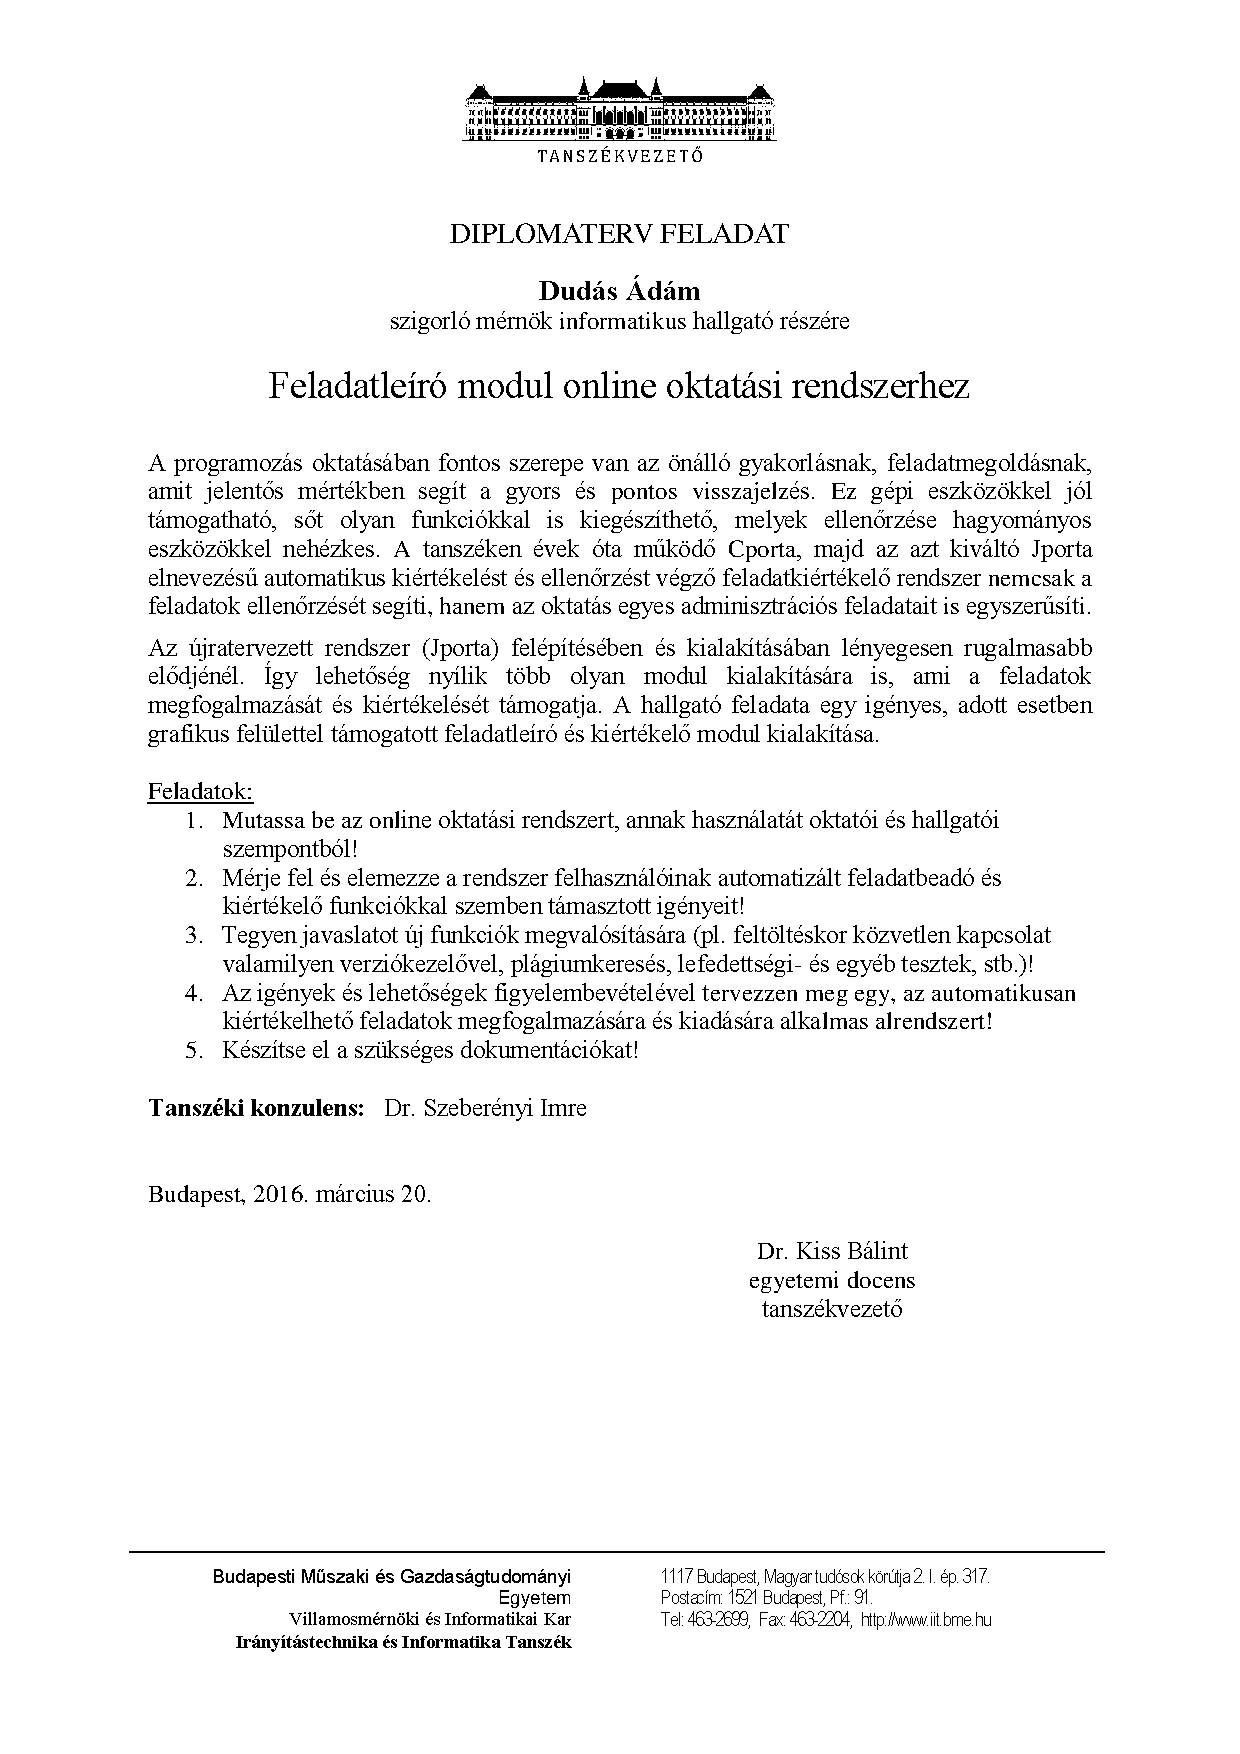
\includepdf[pages={1}]{feladatkiiras.pdf}
%--------------------------------------------------------------------------------------
%	The title page
%--------------------------------------------------------------------------------------
\begin{titlepage}
\begin{center}

\includegraphics[width=60mm,keepaspectratio]{figures/BMElogo.png}\\
\vspace{0.3cm}
\textbf{Budapesti M�szaki �s Gazdas�gtudom�nyi Egyetem}\\
\textmd{Villamosm�rn�ki �s Informatikai Kar}\\
\textmd{\viktanszek}\\[5cm]

\vspace{0.4cm}
{\huge \bfseries \vikcim}\\[0.8cm]
\vspace{0.5cm}
\textsc{\Large \vikdoktipus}\\[4cm]

\begin{tabular}{cc}
 \makebox[7cm]{\emph{K�sz�tette}} & \makebox[7cm]{\emph{Konzulens}} \\
 \makebox[7cm]{\vikszerzo} & \makebox[7cm]{\vikkonzulens}
\end{tabular}

\vfill
{\large \today}
\end{center}
\end{titlepage}



%--------------------------------------------------------------------------------------
% Nyilatkozat
%--------------------------------------------------------------------------------------
\begin{center}
\large
\textbf{HALLGAT�I NYILATKOZAT}\\
\end{center}

Alul�rott \emph{\vikszerzo}, szigorl� hallgat� kijelentem, hogy ezt a szakdolgozatot/ diplomatervet \textcolor{blue}{(nem k�v�nt t�rlend�)} meg nem engedett seg�ts�g n�lk�l, saj�t magam k�sz�tettem, csak a megadott forr�sokat (szakirodalom, eszk�z�k stb.) haszn�ltam fel. Minden olyan r�szt, melyet sz� szerint, vagy azonos �rtelemben, de �tfogalmazva m�s forr�sb�l �tvettem, egy�rtelm�en, a forr�s megad�s�val megjel�ltem.

Hozz�j�rulok, hogy a jelen munk�m alapadatait (szerz�(k), c�m, angol �s magyar nyelv� tartalmi kivonat, k�sz�t�s �ve, konzulens(ek) neve) a BME VIK nyilv�nosan hozz�f�rhet� elektronikus form�ban, a munka teljes sz�veg�t pedig az egyetem bels� h�l�zat�n kereszt�l (vagy autentik�lt felhaszn�l�k sz�m�ra) k�zz�tegye. Kijelentem, hogy a beny�jtott munka �s annak elektronikus verzi�ja megegyezik. D�k�ni enged�llyel titkos�tott diplomatervek eset�n a dolgozat sz�vege csak 3 �v eltelte ut�n v�lik hozz�f�rhet�v�.

\begin{flushleft}
\vspace*{1cm}
Budapest, \today
\end{flushleft}

\begin{flushright}
 \vspace*{1cm}
 \makebox[7cm]{\rule{6cm}{.4pt}}\\
 \makebox[7cm]{\emph{\vikszerzo}}\\
 \makebox[7cm]{hallgat�}
\end{flushright}
\thispagestyle{empty}

\vfill
\clearpage
\thispagestyle{empty} % an empty page


\tableofcontents\vfill
%----------------------------------------------------------------------------
% Abstract in hungarian
%----------------------------------------------------------------------------
\chapter*{Kivonat}\addcontentsline{toc}{chapter}{Kivonat}

A tanulási folyamatban jelentős szerep jut az önálló gyakorlásnak, feladatmegoldásnak, amelyhez fontos, hogy eredményességéről minél gyorsabb és megbízhatóbb visszajelzést kapjon a tanuló.
Ezt nagyban segítheti, ha a szükséges ellenőrzések minél nagyobb része automatizáltan történik, sok munkát levéve ezzel az oktatók válláról.
A programozás oktatása ebből a szempontból kitüntetett helyzetben van, hiszen a programok helyességének, elvárt működéstől való eltéréseinek vizsgálata már szinte a kezdetektől magas fokú automatizálással történik.

Az utóbbi időben, az online oktatás lehetőségeinek felismerésével, a szélessávú internethozzáférések mindenki számára elérhetővé válásával elterjedtté váltak az oktatást segítő platformok, melyek a hallgatók és az oktatók munkáját a tantermeken kívül is segítik.
Ilyen rendszer a BME Irányítástechnika és Informatika Tanszékén működő JPORTA is, amely a programozás oktatását automatikus feladatkiértékelést és ellenőrzést végző funkciója mellett egyéb adminisztrációs oktatói feladatok támogatásával igyekszik segíteni.

Diplomatervemben bemutatom a JPORTA rendszer működését, és a már említett feladatkiértékelő alrendszer tervezésének lépéseit.
Ez utóbbi részeként ismertetem a modullal szemben támasztott követelményeket, és ez alapján megtervezek egy, az automatizáltan kiértékelhető feladatok leírására alkalmas struktúrát, és az ezzel elkészített feladatokra érkező, hallgatók által készített megoldások kiértékelésére képes rendszert.
Végül javaslatot teszek két új funkció megvalósítására, melyeket röviden részletezek.
\vfill

%----------------------------------------------------------------------------
% Abstract in english
%----------------------------------------------------------------------------
\begin{otherlanguage}{english}
\chapter*{Abstract}\addcontentsline{toc}{chapter}{Abstract}

There is a considerable part in the process of learning that goes to individual practice and problem solving where getting fast and reliable feedback about their progress is essential for students.
This can benefit greatly from doing substancial parts of the necessary verification automatically, freeing educators from significant work.
From this perspective the education of programming is in a special position because validation and testing of programs was performed with high levels of automation from the beginning.

In recent times, with the recognition of potential in online education and the widespread availability of broadband internet connectivity we see the proliferation of platforms supporting education that aid the work of students and teachers outside of the classroom.
JPORTA found at the Department of Control Engineering and Information Technology at BUTE is such a system providing assistance for educators with administrative tasks beside its automatic submisson evaluation and testing facility.

In my master's thesis I'll introduce the operation of JPORTA and the design process of the aformetioned submission evaluation subsystem.
As part of this, I'll present the requirements for the module, than I'll design a structure suitable for the description of automatically evaluable assignments and a system capable of evaluating submissions made by students for assignments created via said structure.
Lastly, I'll suggest two new features which I'll detail briefly.
\end{otherlanguage}
\vfill


%----------------------------------------------------------------------------
\chapter{Bevezető}
%----------------------------------------------------------------------------

% Gyakorlás szerepe a tanulásban
A tanulás egy nehéz és időigényes folyamat, melynek megértésével és tökéletesítésével napjainkban is aktívan foglakozik a tudomány.
Ennek a folyamatnak elengedhetetlen része az önállóan végzett feladatmegoldás, a gyakorlás, mely során az elméleti tudás a gyakorlatban is hasznosítható tapasztalattá válik.
Gyakorlás közben fontos, hogy minél gyakrabban -- ha lehet, folyamatosan -- ellenőrizzük munkánk eredményét, ezzel biztosítva azt, hogy ne keletkezzenek rossz berögződések, melyek utólagos kijavítása további időt igényelne.

Az ellenőrzés módozatait többféle nézőpontból is értékelhetjük.
Az egyik ilyen nézőpont az ellenőrzési módszer flexibilitása, amely azt mutatja meg, mennyire változtatható meg a feladat úgy, hogy az ellenőrzési módszer továbbra is alkalmazható maradjon.
A spektrum egyik végén állnak az inflexibilis módszerek, amilyen például egy adott feladathoz mellékelt megoldókulcs.
A legegyszerűbb megoldókulcsok egyedül a feladat elvárt eredményét adják meg, ezért ezek flexibilitása igen csekély, hiszen a feladatban bármilyen érdemi változtatást elvégezve elvesztik érvényességüket. 
Ugyanakkor ezek a leggyorsabb és legolcsóbb módszerek, hiszen egyetlen összehasonlítás szükséges a saját és a megoldókulcs által megadott érték között, a megoldókulcsok pedig minimális költséggel sokszorosíthatóak és felhasználhatóak.
A spektrum másik végén találhatóak az oktatók -- általános esetben az adott terület szakértői --, akik a feladat témakörében való jártasságuk révén gyakorlatilag bármely megoldás ellenőrzésére képesek.
Az oktató azonban drága erőforrás, mind időben, mind pénzben, hiszen egy adott téma szakértőjeként a tanulók feladatainak ellenőrzése helyett az iparban is nagy szükség lenne rá.
Ebből fakadóan -- sok oktató alkalmazása költséges, ugyanakkor az iparnak nagyszámú szakértőre van szüksége -- az egy oktatóra eső hallgatók száma igen magas, amely körülmény nem kedvez az oktatás színvonalának, hiszen így minden hallgatóra kevesebb ideje jut az oktatónak.
Ha a spektrum két végének előnyeit -- könnyű sokszorosíthatóság, gyors működés, de magasabb szintű flexibilitás szakértelem hozzáadásával -- összehozzuk a számítástechnika által nyújtott automatizálási lehetőségekkel, eljuthatunk az \textit{automatizált feladatkiértékelő rendszerek} ötletéhez.


\section{Automatizált feladatkiértékelés}

\section{Online oktatást segítő rendszerek}
% TODO: Feladat indokoltsága: miért/mire jók az online oktatási rendszerek, a feladatbeadó rendszerek, automatikus kiértékelés
%       Eddigi megoldások (Coursera, Khan Academy, edX, Cporta)[http://www.lifehack.org/articles/money/25-killer-sites-for-free-online-education.html], hallgatói és oktatói szemszög


\section{A diplomaterv felépítése}
A dolgozatot az elvégzett munka és továbbfejlesztési lehetőségek összefoglalásával zárom.

%----------------------------------------------------------------------------
\chapter{A Jporta}\label{chapter:jporta}
%----------------------------------------------------------------------------

A Jporta a Budapesti Műszaki és Gazdaságtudományi Egyetem (továbbiakban: BME) Irányítástechnika és Informatika Tanszékén (továbbiakban: IIT) működő, a BME Közigazgatási Informatikai Központ (továbbiakban: BME IK vagy IK) által fejlesztett, oktatást támogató portál, mely a fő funkcióját képző feladatbeadó és -kiértékelő rendszeren kívül az oktatással kapcsolatos adminisztrációs feladatokban (pl. jelenlét vezetése, hallgatók értékelése, üzenetváltás felhasználók között) is segíteni igyekszik felhasználóit.

Ugyan a Jporta fejlesztése csak 2013-ban kezdődött, a tanszéken már 2008 óta használják az eredetileg prototípusnak készült Cporta rendszert, mely minden szempontból a Jporta elődjének tekinthető.

\section{Cporta -- a prototípus}
A Cporta feladatbeadó és gyakorló rendszer a nevéhez illően kifejezetten a C és C++ nyelvek oktatásához lett kifejlesztve.
A portálon a hallgatóknak lehetősége van a kiadott feladatokra C és C++ nyelven íródott programkódok feltöltésére, melyeket a rendszer lefordít, futtat, és teszteléssel értékel.
Lehetőség van emellett fordítást nem igénylő fájlok feltöltésére is (pl. dokumentáció, bemeneti fájlok a teszteléshez).
A Cporta ezen kívül tanulmányi rendszer jellegű funkciókat is megvalósít: kezeli a hallgatók eredményeit és a jelenléti íveket is.
\cite{Ory13}
\begin{figure}
    \centering
    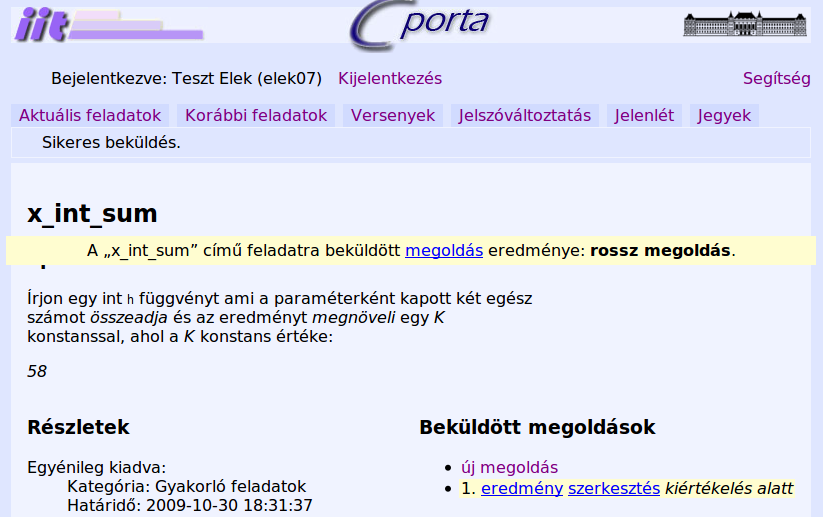
\includegraphics[width=\textwidth]{figures/Cporta}
    \caption{A Cporta felülete}
\end{figure}
A ezeket a funkciókat a Jporta bevezetéséig továbbra is a Cporta látja el \textit{A programozás alapjai 2.} tárgy esetében.

\subsection{A Cporta működése}
A Cportán -- ahogy az oktatásban általában -- a feladatokat az oktatók készíthetik el.
A feladatok több részből állnak:
\begin{itemize}
    \item metaadatok (cím, szerző, fordítási paraméterek, futtatási korlátozások, stb.)
    \item specifikáció (a feladat leírása HTML formában)
    \item oktató által megadott fájlok
    \item tesztesetek
\end{itemize}
A feladat specifikációja lehet statikus, vagy a hallgató adatai alapján dinamikusan generált, így lehetőség van hasonló, ám hallgatónként egyedi feladatok készítésére.
Az oktató által megadott fájlok lehetnek nyilvánosak (pl. a használható függvények fejléceit tartalmazó állomány), vagy rejtettek (pl. a teszteléshez használt bemeneti adatfájlok).
A tesztesetek a fordítási lépés eredményeként kapott futtatható állományon hajtódnak végre.
A specifikációhoz hasonlóan kétféle változatuk lehetséges.
Egyszerűbb esetben megadhatunk egy statikus bemenetnél elvárt statikus választ vagy kilépési kódot, amit a teszteset ellenőriz.
Összetettebb esetben megadhatunk két futtatható parancsállományt: az egyik előkészíti a futtatási környezetet és a szabványos bemenetet, a másik ellenőrzik a futás utáni környezetet, kimenetet és kilépési kódot.
\cite{Ory13}

A kiadott feladatokra a hallgatók megoldásokat küldhetnek be, melyeket a rendszer a lehető leghamarabb kiértékel.
A megoldások tartalmazhatnak C és C++ nyelvű forrásállományokat, a tesztelés során elérhető adatállományokat, illetve dokumentációs fájlokat.
A webportálra feltöltött megoldások egy központi ütemezőn keresztül kerülnek a kiértékelést végző végrehajtó gépre.
A kiértékelés végén a végrehajtó gép az eredményeket visszaküldi a webportálra, amely megjeleníti azokat a felhasználóknak. 

A Cporta eredetileg az online, elektronikus feladatkiadás és -beadás oktatásban való használatának vizsgálatára, a koncepció működésének bizonyítására készült.
Ez a prototípus azonban nem hosszútávú használatra lett tervezve, továbbá a használat során felmerülő igényekre válaszként tervezett és beépített kiegészítések a fejlesztésükre szánt idő és erőforrások hiányában -- és ebből következően megfelelő tesztelés és dokumentáció nélkül -- rontották a rendszer stabilitását és karbantarthatóságát.  
A portál üzemeltetését végzők egyöntetű döntése nyomán 2013-ban elindult a Cporta utódjának fejlesztése, eredetileg \textit{swd} néven.

\section{Jporta -- válasz az igényekre}
A Jporta fejlesztésekor az összes Cportával megszerzett tapasztalat a fejlesztők rendelkezésére állt.
A fejlesztéseket 2013-ban Őry Máté kezdte meg szakdolgozata részeként, melyben részletesen elemezte a régi rendszer hiányosságait és az új rendszerrel szemben támasztott követelményeket (lásd \cite{Ory13}).
Munkája részeként ezek alapján megtervezte és elkészítette az új rendszer pilot változatát.  
Ez a változat a feladatkiértékelő funkciónak egy, a Cportáéhoz hasonló, egyszerű változatát valósította meg.
A munka értékelésekor a projekt vezetői arra a döntésre jutottak, hogy a pilot feladatkiértékelő funkciójának felépítése túlságosan merev, néhány használati eset megvalósítására nem, vagy csak nehezen alkalmas. 
Ekkor a portál fejlesztését az IK Cloud csapatának tagjai -- köztük jómagam -- vették át.
Az én feladatom a feladatok leírását és kiadását, és az azokra érkező megoldások beadását és értékelését lehetővé tevő modul továbbfejlesztett modelljének kidolgozása lett, míg a felhasználói felület és az egyéb adminisztrációs funkciók tervezését és implementációját Kálmán Viktor végezte (lásd \cite{Kalman14}).

Az Őry Máté által újratervezett portál sok tekintetben szakított a Cportában felhasznált technológiákkal.
Az új rendszer implementálásához a Python programnyelv 2-es változatát válaszotta, melyet a későbbiekben a 3-as változatra frissítettünk, ezzel biztosítva a szoftver alapját képző komponens tartós támogatottságát, amit már \cite{Kalman14} is említ.
% TODO Django 1.8.9

% TODO flexibilisebb, általánosabb felépítés, több nyelv támogatása, akár nem programozási feladatok támogatása is

\section{A portál használata}
Ahogy azt az előzőekben láthattuk, a portál sok szolgáltatást nyújt felhasználói számára. 
Ezeket a felhasználókat 4 csoportra oszthatjuk: vendégek (nem azonosított felhasználók), hallgatók, oktatók, illetve az adminisztrátorok.
Mivel a tanszéken sok doktorandusz és demonstrátor is végez oktatási tevékenységet, egy felhasználó szerepelhet bizonyos tárgyaknál oktatóként, míg másoknál hallgatóként.
A portál vendégek számára -- jelenleg -- nem tartalmaz hozzáférhető tartalmat, így a még be nem jelentkezett felhasználókat a belépőoldal fogadja.
A belépőoldalon a felhasználók azonosítására két lehetőség van: eduID (egyetemi SSO) vagy a hagyományos felhasználónév--jelszó páros (lásd \figref{jporta-login}).
\begin{figure}[h]
    \centering
    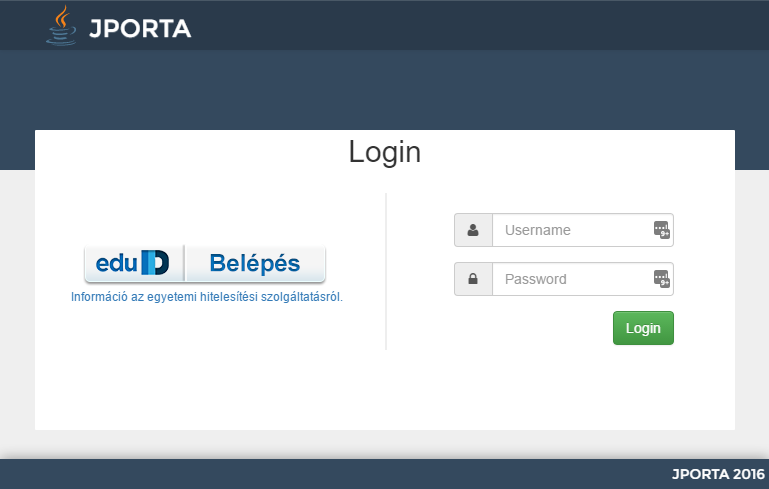
\includegraphics[width=\textwidth]{figures/Jporta-login}
    \caption{A Jporta belépőoldala}
    \label{figure:jporta-login}
\end{figure}
Belépés után a felhasználókat egy kezdőoldal fogadja, melyen a fontosabb információk (pl. aktív és korábbi feladatok, kézi beavatkozást igénylő feladatok) gyűjteménye található.
Már a kezdőoldalon látható (\figref{jporta-home-h}, \figref{jporta-home-o}), hogy a különböző felhasználói szerepek különböző funkciókat tesznek elérhetővé a rendszerben.
Mivel ezek az eltérések egy adott felhasználói szerepkörre (hallgató, oktató, adminisztrátor) jellemzőek, ezért ezeket a nézöpontokat és a hozzájuk kapcsolódó funkciókat az alábbiakban külön részletezem.

\subsection{A portál használata hallgatói szemszögből}
\begin{figure}[h]
    \centering
    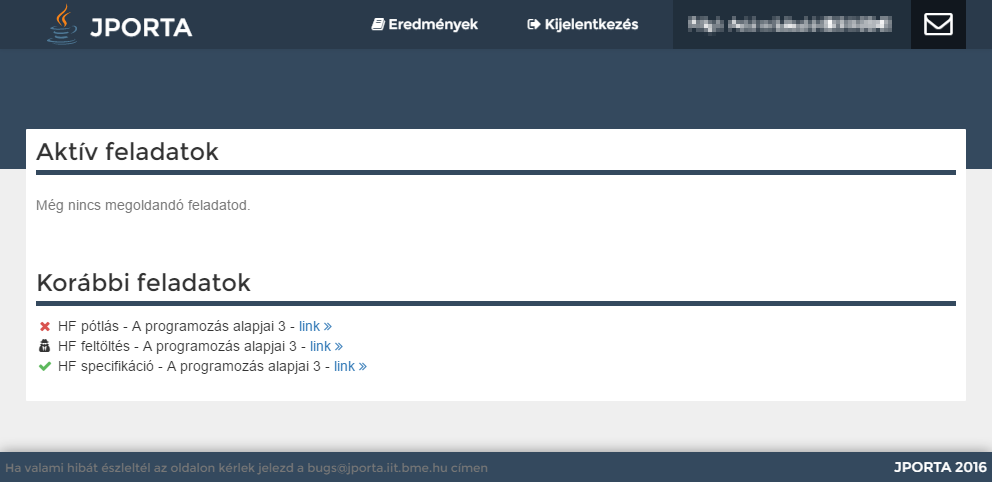
\includegraphics[width=\textwidth]{figures/Jporta-home-h}
    \caption{Jporta kezdőlap (hallgató)}
    \label{figure:jporta-home-h}
\end{figure}
\begin{figure}[h]
    \centering
    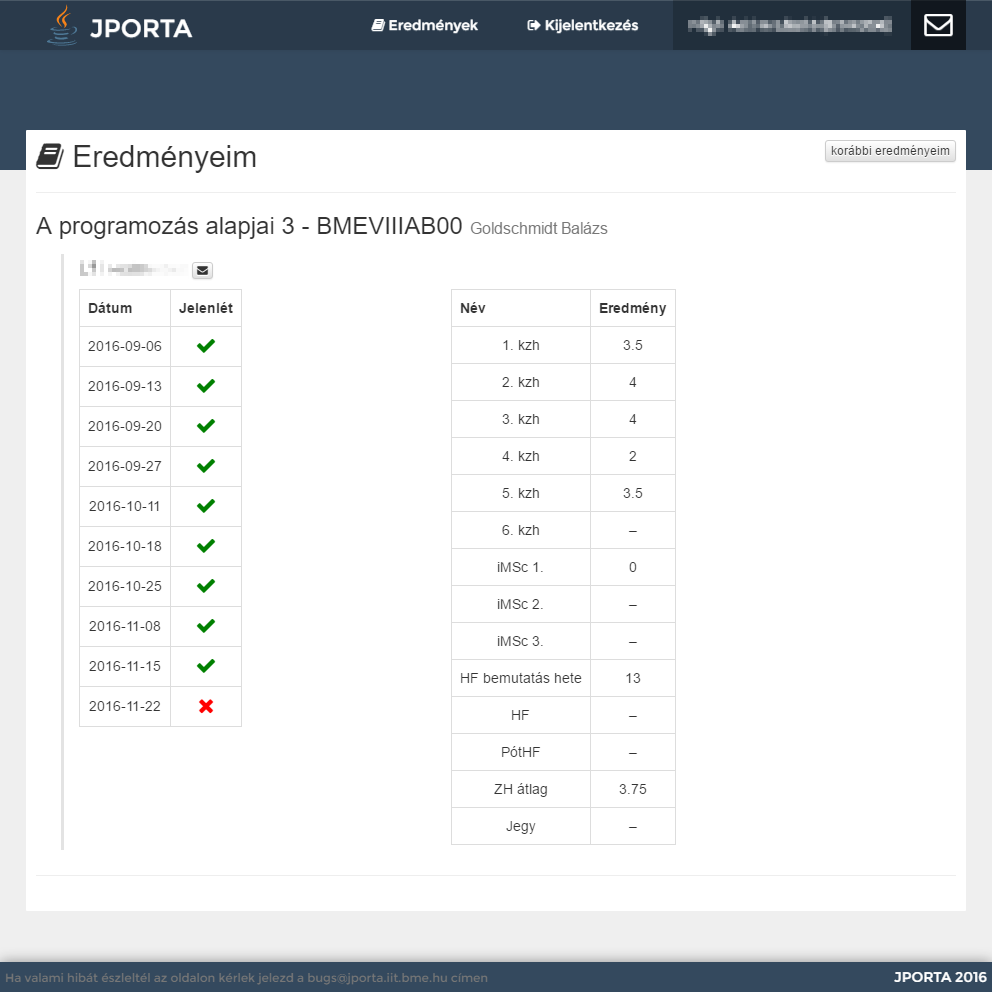
\includegraphics[width=\textwidth]{figures/Jporta-results}
    \caption{Eredményeim oldal}
    \label{figure:jporta-results}
\end{figure}

\subsection{A portál használata oktatói szemszögből}
\begin{figure}[h]
    \centering
    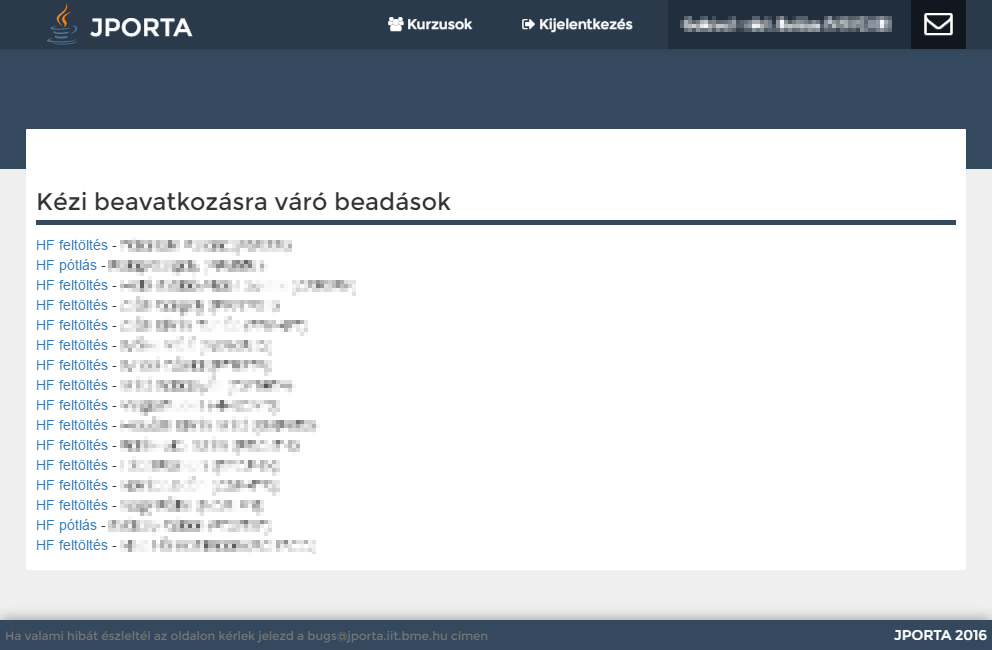
\includegraphics[width=\textwidth]{figures/Jporta-home-o}
    \caption{Jporta kezdőlap (oktató)}
    \label{figure:jporta-home-o}
\end{figure}


\subsection{Adminisztrátori felületek}
Az adminisztrátori jogkörrel rendelkező felhasználók számára elérhető az \textit{Irányítópult} (Management dashboard), ami a \ref{figure:jporta-management-dashboard}. ábrán látható.
Erről a felületről elérhető és kereshető az összes ismert felhasználó listája, illetve itt történik a szemeszterek adminisztrálása is.
A \textit{Szemeszter} szekcióban láthatóak az eddig létrehozott szemeszterek, kezdő- és végdátumaikkal együtt, valamit egy szemléltető diagram ezekről az időszakokról.
Itt hozhatunk létre új szemesztereket, vagy ha szükséges, törölhetjük is őket. 
A jobb felső sarokban található \textit{Django admin} gomb átvezet a Django keretrendszer beépített adminisztrációs felületére, melyről részletesebb leírást \cite{DjangoAdmin} ad.
\begin{figure}[h]
    \centering
    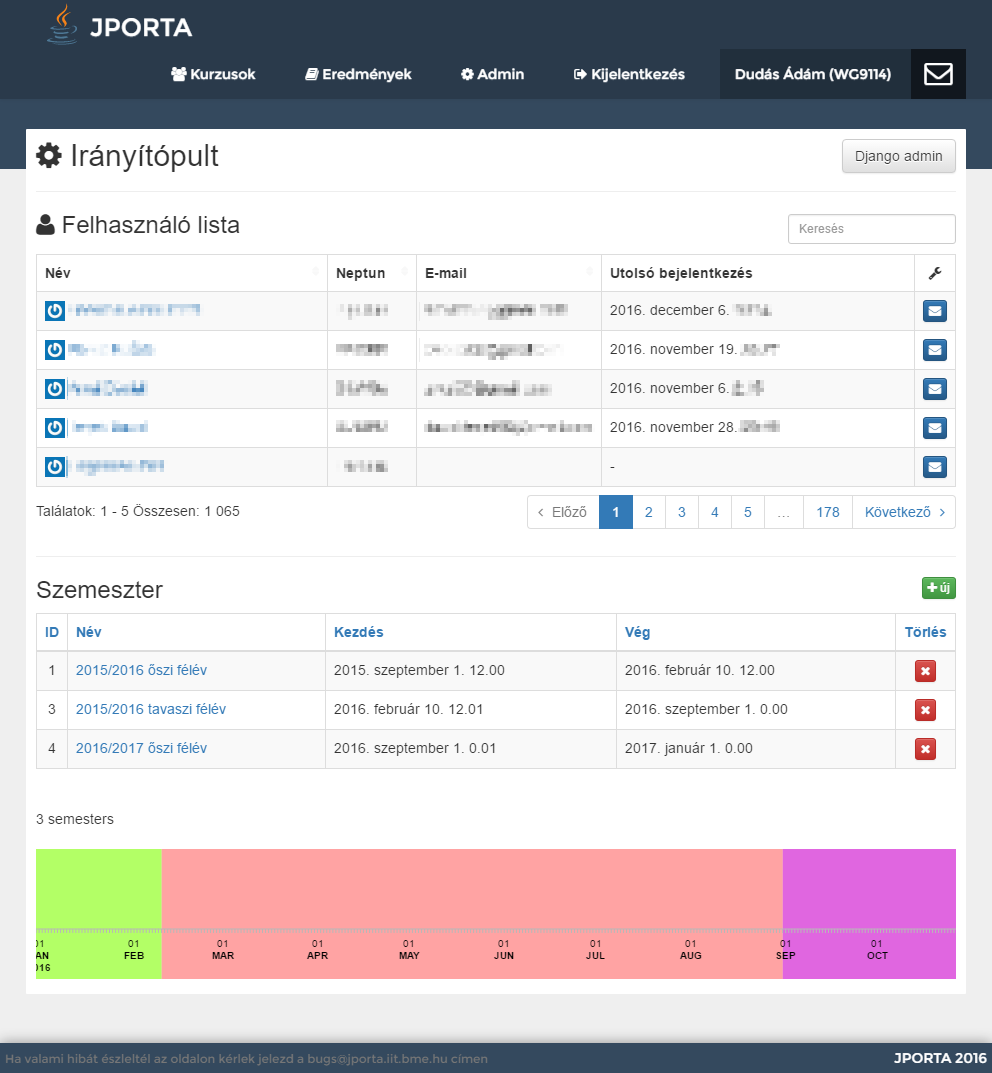
\includegraphics[width=\textwidth]{figures/Jporta-management-dashboard}
    \caption{Irányítópult}
    \label{figure:jporta-management-dashboard}
\end{figure}

\sectsep

% Üzenetküldés
Az összes felhasználó számára rendelkezésre áll továbbá egy beépített üzenetküldés funkció, amelynek segítségével anélkül tudnak egymásnak üzenni a felhasználók, hogy ismerniük kellene címzettük, címzettjeik e-mail címeit.
Minden felhasználó megtekintheti a beérkezett üzeneteit a portál dedikált felületén (\figref{jporta-inbox}), de ha rendelkezik megadott e-mail címmel, akkor az üzenetek erre a címre is továbbításra kerülnek, sőt, a rendszer érzékeli, ha a levelet egy külső levelezőben olvasta a felhasználó, és azt belül is olvasottnak nyilvánítja.
\begin{figure}[h]
    \centering
    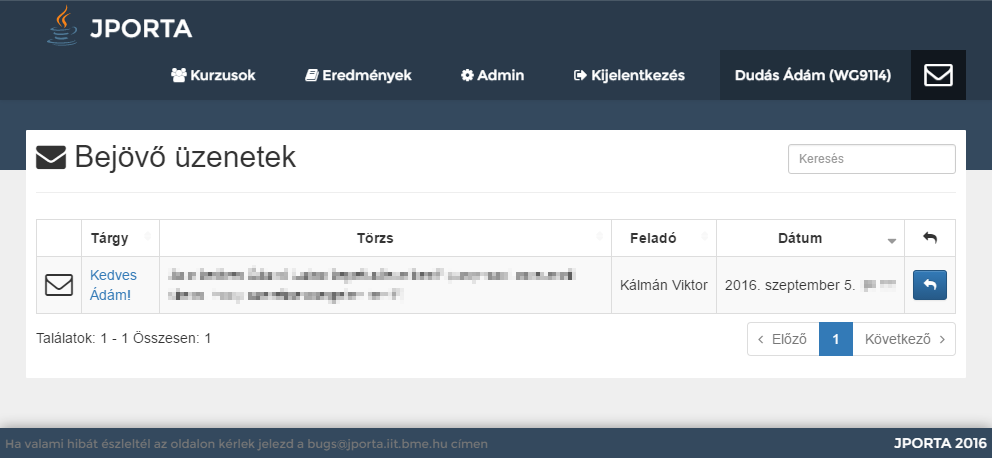
\includegraphics[width=\textwidth]{figures/Jporta-inbox}
    \caption{Bejövő üzenetek}
    \label{figure:jporta-inbox}
\end{figure}
A tárgyért felelős oktatók a tárgy oldalán található \textit{Üzenetek} fül alatt akár az egész kurzusnak vagy bizonyos kurzuscsoportoknak is küldhetnek üzeneteket (\figref{jporta-course-messages}).
Ehhez hasonlóan a kurzuscsoportok oktatói is tudnak üzenetet küldeni saját csoportjaiknak.
\begin{figure}[h]
    \centering
    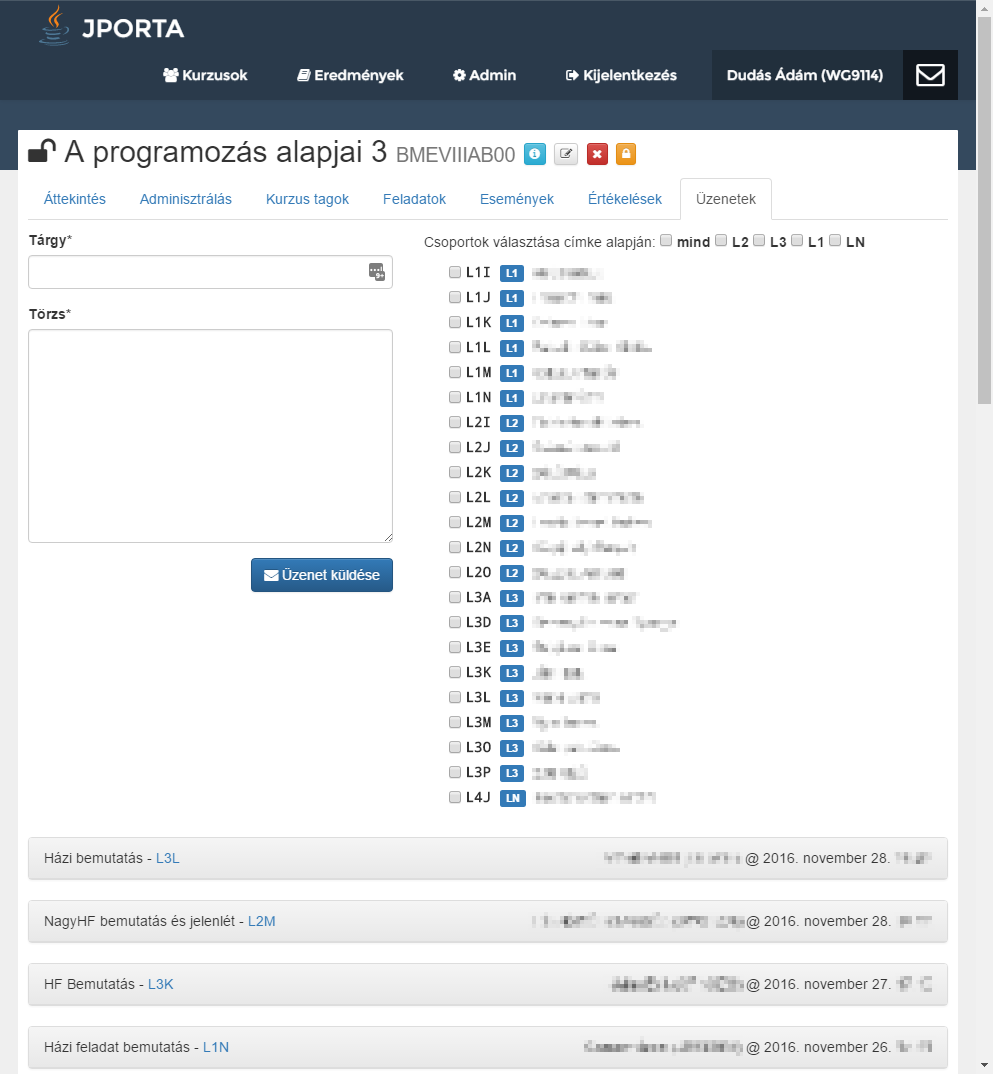
\includegraphics[width=\textwidth]{figures/Jporta-course-messages}
    \caption{Kurzus szintű üzenetküldés}
    \label{figure:jporta-course-messages}
\end{figure}

%----------------------------------------------------------------------------
\chapter{Automatizált feladatkiértékelő modul}\label{chapter:exercise}
%----------------------------------------------------------------------------

A Jporta legfőbb alkotóeleme a feladatok leírásáért és a kiadott feladatokra érkezett megoldások automatizált kiértékeléséért felelős modul.
A portálnak ebben az újabb változatában fontos cél, hogy ez az alrendszer flexibilisebb legyen, mint az eddigi megoldások.
Ezt a flexibilitást egy általánosabb, de mégis egységes felépítés alkalmazásával igyekeztem elérni.
Az általam megtervezett rendszer a programnyelvek használatához kapcsolódó eszközök (pl. fordítók, interpreterek, tesztelési környezetek) alacsonyszintű működését egy közös, magasabb szintű absztrakció mögé rejti, melynek hatására a rendszer bővíthetősége megnő, és akár nem programozási jellegű feladatok készítésére is alkalmassá válik.

Ebben a fejezetben végigvezetem az olvasót a modul megtervezésének folyamatán, a követelmények összegyűjtésétől a megtervezett rendszer működésének és használatának leírásán át, egészen az implementációhoz szükséges technológiák bemutatásáig.

\section{Követelmények}\label{section:requirements}
A tervezés első lépése a tervezendő modullal szemben támasztott követelmények felmérése, amit a már meglévő munka elemzésével kezdtem.
A modul követelményeinek túlnyomú részét \cite{Ory13} már azonosította, miközben a portál egészére nézve végezte el ezt a feladatot.
A \cite{Kalman14} szakdolgozat tovább pontosította a követelményeket, miközben a portál más aspektusainak fejlesztésén dolgozott.
Az általuk feltárt követelmények a következők:
\begin{enumerate}
    \item A hallgató listázhatja és megtekintheti a számára kiosztott feladatokat.
    \item A hallgató a feladatokhoz megoldást adhat be.
    \item A hallgató megtekintheti korábban beadott megoldásait és azok eredményeit.
    \item Az oktató új feladatot hozhat létre.
    \item \label{req:specification} A feladatok tartalmaznak feladatkiírást, amely lehet statikus vagy dinamikusan generált.
    \item A feladatoknak része lehet egy vagy több fájl, amelyeket az oktató ad meg.
    \item A feladatoknak része lehet egy vagy több fájl, melyet a hallgatónak kell beadnia.
    \item A feladatok tartalmaznak automatikusan végrehajtható ellenőrzéseket.
    \item Az oktató feladatot adhat ki hallgatónak.
    \item Az oktató a feladatra beadott megoldásokat listázhatja, megtekintheti azok tartalmát, eredményét.
    \item A rendszer bővíthető új nyelvek, környezetek, eszközök támogatásával.
    \item Egy feladatkörben több alternatív eszköz (pl. GCC és Clang C fordítók) támogatása, akár egy feladaton belül is.
    \item \label{req:isolation} A megoldások kiértékelése izolált környezetben történik.
    \item \label{req:distributed} A kiértékelés elosztott rendszerben, tetszőleges számú gépen működik.
\end{enumerate}
Ezek a követelmények részben megegyeznek a Cporta eredeti követelményeivel, illetve tartalmaznak a Cporta használata közben megfogalmazott igényeket is.
A Jporta első, demó változatának próbája során azonban további igények fogalmazódtak meg a felhasználókban, melyek a feladatkiértékelő modult is érintették.
Ezek alapján én az alábbi kiegészítéseket teszem a követelmények már meglévő listájához:
\begin{enumerate}[resume]
    \item \label{req:manual} A feladatok tartalmazhatnak emberi beavatkozást igénylő ellenőrzéseket.
    \item \label{req:traceability} A kiértékelés folyamata legyen nyomonkövethető.
\end{enumerate}

A követelmények nagy része nem igényel magyarázatot, ám van néhány, amelyekről szeretnék még pár szót szólni.

Az \ref{req:specification}. követelmény a feladatkiírás szövegének dinamikus generálhatóságát írja elő.
Ez azt jelenti, hogy a feladatkiírás hallgatónként eltérő lehet, amely eltérés a hallgató személyétől, pontosabban a személyéhez kapcsolódó, rendelkezésre álló információktól függ.
Ilyen adat lehet például a hallgató neve, Neptun kódja, e-mail címe, felhasználóneve, stb.
Ezenkívül, a generáláshoz felhasználható bármilyen, a generálás pillanatában rendelkezésre álló erőforrás, pl. az oktató által megadott fájl, kerülendő azonban a nem megismételhető műveletekkel szerezhető adatok felhasználása (pl. aktuális idő lekérdezése, az operációs rendszer véletlenszám generátorának használata).

A \ref{req:isolation}. követelmény előírja, hogy a feladatok kiértékelése izolált környezetben történjen.
Ez nagyon fontos kitétel a rendszer biztonsága és stabilitása szempontjából.
Az izoláció egyrészt védi a gazda rendszert, amelyben a kiértékelések végbemennek, másrészt az egyidejűleg futó kiértékeléseket is védi egymástól.

A \ref{req:manual}. követelményre azért van szükség, mert a informatika jelenlegi eszközeivel nem minden ellenőrzés valósítható meg, néha elkerülhetetlen az emberi beavatkozás szükségessége.
A rendszer előző változataiban azonban nem volt ilyen jellegű funkció, a kiértékelés minden lépése automatizáltan történt.
Ez az új igény azonban jelentős változással jár a kiértékelés menetében, ugyanis egy potenciálisan végtelen, de mindenképp az eddigiekhez képest hosszú várakozást -- max. pár 100 milliszekundum kontra percek, órák, napok -- iktat be a folyamatba.
Ahhoz, hogy ezalatt a várakozás alatt a kiértékelést végző rendszer erőforrásai ne legyenek feleslegesen lefoglalva, a kiértékelés végrehajtása nem történhet egyetlen folytonos menetben, szükség van a folyamat állapotának elmentésére, majd visszatöltésére és a kiértékelés folytatására az emberi beavatkozás elvégzése után.

A \ref{req:traceability}. követelményre a rendszer auditálhatósága miatt van szükség, de a feladatokban, esetleg a feladatot kiértékelő rendszerben előforduló hibák feltárását és kezelését is megkönnyíti.
A követelmény teljesítéséhez rendelkezésünkre kell állnia a kiértékelés mindenkori állapotának, illetve a kiértékelés során keletkezett részeredményeknek.

\section{A feladatkiértékelő modul működése}\label{section:execution-procedure}
Az újratervezett feladatkiértékelő modul felépítését a \textit{csővezetékek és szűrők} (\textit{pipes and filters}, \cite{PipesAndFilters}) architektúrális tervezési mintára alapoztam.
A \textit{szűrők} a feladatok kiértékelési lépéseit (pl. fordítás, futtatás, tesztelés) reprezentálják, míg a \textit{csővezetékek} a lépések közötti adatáramlást.
A \ref{figure:example-pipeline}. ábrán a leggyakrabban előforduló feladat felépítés sematikus képe látható, melyen a különféle ``dobozok'' testesítik meg a szűrőket, a köztük vezető nyilak pedig a csővezetékeket, melyek egyúttal az adatáramlás irányát is szemléltetik.
Ahogy az ábrán is jól látható, a szűrőket három csoportra oszthatjuk: \textit{források}, \textit{átalakítók} és \textit{nyelők}.
Az ábrán látható paralelogrammák a források, a téglalapok az átalakítók, a hengerek pedig a nyelők.

\begin{figure}[h]
    \centering
    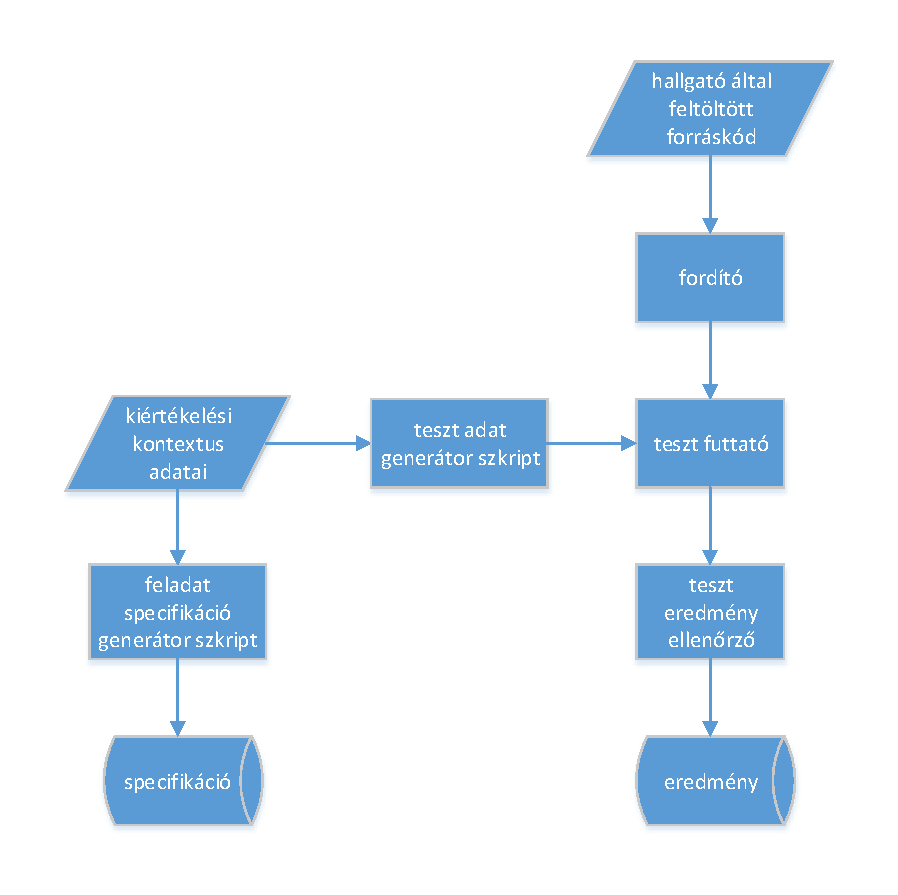
\includegraphics[width=0.95\textwidth]{figures/example-pipeline}
    \caption{A legjellemzőbb feladatstruktúra}
    \label{figure:example-pipeline}
\end{figure}

Az így felépített struktúra mindig egy irányított gráfot határoz meg, melynek csúcsai a szűrők, élei pedig a csővezetékek, az élek iránya pedig a szűrők közti adatáramlás iránya.
Ha ennek a gráfnak az éleit megfordítjuk, egy \textit{függőségi gráfot} kapunk, melynek segítségével meghatározhatjuk a kiértékelés lépéseinek sorrendjét.
Ahhoz, hogy a feladat kiértékelhető legyen, \textbf{a függőségi gráfnak körmentesnek kell lennie}. \cite{wiki:DependencyGraph}

A kiértékelés kezdetben mindig a függőségi gráf egy 0 bemeneti fokszámú csúcsából -- az eredeti gráfban nyelő -- indul.
A következő lépés, hogy meghatározzuk azon csúcsok halmazát, amelyektől a kiértékelendő csúcsunk közvetlenül függ.
Mielőtt ezt a csúcsot kiértékelhetnénk, az összes ebben a halmazban lévő csúcsnak ki kell lennie értékelve, ezért ezt az algoritmust a halmaz elemeire is rekurzívan alkalmazzuk.
Ha olyan csúcsot találunk, amelynek nincs függősége -- azaz, 0 a kimeneti fokszáma; az eredeti gráfban forrás --, akkor azt a csúcsot azonnal kiértékelhetjük.
Mivel a gráfról kikötöttük, hogy körmentesnek kell lennie, csúcsainak száma pedig véges, az algoritmusunk véges számú lépésben kiértékeli a feltárt részgráfot.
Ez az algoritmus soros végrehajtás esetén ideális.
A kiértékelés hatékonysága növelhető, ha a már kiértékelt csúcsok eredményeit egy gyorsítótárban eltároljuk, így ha több csúcs is függ ugyanattól az eredménytől, a kiértékelést akkor is csak egyszer végezzük el (lásd \cite{wiki:Memoization}).

Egy másik lehetséges algoritmus, ha a függőségi gráfot a lehető legkevesebb szintre osztjuk úgy, hogy az egy szinten lévő csúcsok között ne legyen függőség.
Az azonos szinten lévő csúcsok egymástól függetlenül kiértékelhetőek, amit kihasználhatunk, ha lehetőségünk van párhuzamos végrehajtásra.

A ``pipe'' és ``filter'' szavakat az informatikában sok esetben használják, gyakran hasonló, de eltérő jelentésekkel.
Ezzel összhangban a Python nyelvben a ``filter'' szó egy beépített függvényre hivatkozik, és a ``pipe'' szó is sok beépített függvénykönyvtárban előfordul.
A félreértések elkerülése végett a továbbiakban a szűrőket \textit{blokkoknak} (\textit{block}), a csővezetékeket pedig \textit{azonosítóknak} (\textit{handle}) fogom nevezni.
Ez azért is előnyös, mert a szóhasználat jobban utal a minta konkrét megvalósítására, amely jobban hasonlít a matematikai feladványokból ismert ``műveleti gépekhez''.

\section{Feladatok leírása}
Az előzőekben vázoltak alapján, szinte adja magát a feladatok leírására szolgáló modell, melynek két központi eleme a \texttt{Block} és a \texttt{Handle} osztályok.
A \texttt{Block} absztakt ősosztályként szolgál a különböző funkciókat (pl. fájlfeltöltés, fordítás, futtatás, ellenőrzés) megvalósító blokk osztályok számára.
Az ezekből példányosított blokkok pontosan egy feladatnak részei, melyet az \texttt{Exercise} osztály modellez.
A blokkokat a \texttt{Handle} osztály példányai kötik össze, melyek egy feladaton belül egyedi névvel rendelkeznek.
Ez az összeköttetés azonban nem közvetlen, hanem a \texttt{Provider} és a \texttt{Consumer} osztályok példányain keresztül történik.
Minden \texttt{Handle} példány pontosan egy \texttt{Provider} példányhoz tartozik, amelyek szintén pontosan egy blokkhoz tartoznak.
Ez a kapcsolat jelzi, hogy melyik blokk kiértékelése állítja elő az azonosító által megnevezett erőforrást, vagyis ezek a blokk kimenetei.
A \texttt{Consumer} osztály példányai ennek a kapcsolatnak a párját testesítik meg, vagyis hogy az erőforrást mely blokkok használják fel kiértékelésükkor, mik a blokk bemenetei.
Minden \texttt{Consumer} példány pontosan egy blokkhoz kapcsolódik, ám egy \texttt{Handle} példányhoz több \texttt{Consumer} is kapcsolódhat, hiszen ugyanazt az erőforrást több blokk is felhasználhatja.
Minden blokkra igaz, hogy nulla vagy több \texttt{Provider} és \texttt{Consumer} példányhoz kapcsolódik.
Az előző részekben említett \textit{források} azok a blokkok lesznek, amelyek nem kapcsolódnak \texttt{Consumer} példányhoz.
Hasonlóképp, a \texttt{Provider}-ektől mentes blokkok lesznek a \textit{nyelők}.
Az itt leírt modellosztályokat szemléltető UML osztálydiagram a \ref{figure:exercise-uml-cd}. ábrán látható.

\begin{figure}[h]
    \centering
    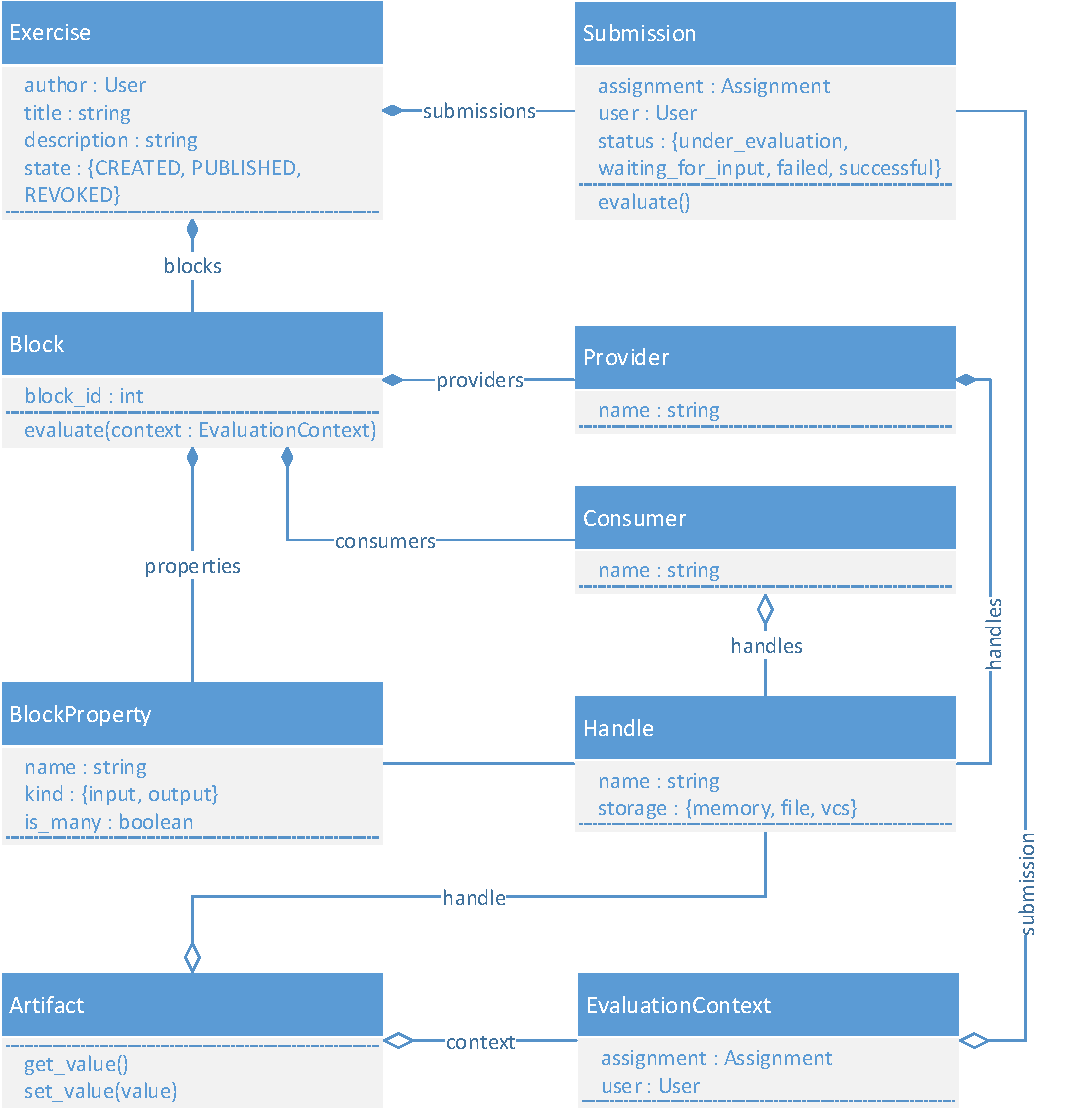
\includegraphics[width=\textwidth]{figures/exercise-uml-cd}
    \smallskip
    \caption{Feladatleíró modul UML osztálydiagramja}
    \label{figure:exercise-uml-cd}
\end{figure}

Mivel a \texttt{Block} osztály csak ősként szolgál a különböző blokktípusok számára, minden egyedi funkciót az ebből származtatott osztályokban kell megvalósítani.
A blokkok be- és kimeneteit a \texttt{Block\-Property} osztály példányai jelölik a Django modellek \texttt{Field}-jeihez hasonló, deklaratív megoldással.
Amikor a Python értelmező betölti a \texttt{Block} osztály egy leszármazottját, a típus létrehozásának folyamatába beavatkozik a \texttt{Block\-Metaclass} osztály, ami a Python \texttt{\_\_new\_\_} speciális metódusát definiálja felül, és a \texttt{Block} osztály meta\-class-aként van megjelölve. \cite{PythonMetaclass}
Ez a metódus a típus definiciójában található összes \texttt{Block\-Property} típusú attribútumot lecseréli egy \texttt{Block\-Property\-Descriptor} típusú attribútumra, aminek átadja az attribútum nevét és paramétereit, illetve a típus egy speciális attribútumába feljegyzi a tulajdonság nevét.
Ez utóbbi lista alapján tudja azonosítani a blokk osztály, hogy mely attribútumai be- és kimenetek.
A \texttt{Block\-Property\-Descriptor} példányok a Python nyelv \textit{leíró} (\textit{descriptor}) mintáját valósítják meg.
Ez az osztály ugyan felüldefiniálja a mintában található mindhárom speciális metódust (\texttt{\_\_get\_\_}, \texttt{\_\_set\_\_} és \texttt{\_\_delete\_\_}), azonban csak a \texttt{\_\_get\_\_} metódust valósítja meg.
Ez a következő speciális működést vonja magaután: amikor egy blokk osztály példányának be- vagy kimenetet reprezentáló attribútumát elérjük (értsd: \texttt{blokk\_peldany.attributum}), akkor ez a felüldefiniált \texttt{\_\_get\_\_} metódus hívódik meg úgy, hogy a leírót, a blokk példányt és a blokk típust (osztályt) kapja meg paraméterül. \cite{PythonDescriptors}
Ez a metódus a \texttt{Block\-Property\-Instance} osztály egy példányával tér vissza.
Ez az objektum az eredeti \texttt{Block\-Property} paraméterein és a hozzá vezető attribútum nevén kívül magára a tartalmazó blokk példányra is tartalmaz egy referenciát, amelyen keresztül manipulálni tudja azt.

A blokkok egyedi kiértékelési algoritmusát a leszármazott osztály \texttt{evaluate} metódusa valósítja meg.
Ez a metódus paraméterként megkapja a blokk referenciáját és a blokk kiértékelésének kontextusát (lásd \ref{section:submission-evaluation}. szakasz), és ezeket felhasználva elvégzi a kimeneti értékei kiszámításához szükséges számításokat, majd a kontextusban beállítja a kimeneteinek megfelelő értékeket.

\section{Feladatok készítése}\label{section:exercise-creation}
A rendszer, általános felépítése miatt, nem tartalmaz sok megkötést a leírható feladatokra: az egyszerű PDF formátumú beadandók feltöltéstől egészen egy grafikus felülettel rendelkező, interaktív házi feladatokat fordító, futtató és tesztelő beadásokig szinte bármilyen feladat összeállítható benne.
Ahhoz, hogy ez a változó komplexitású munkafolyamat felhasználóbarát maradjon, egy egyszerű felületre van szükség, amely nagy összetettségű feladatok esetén sem válik kezelhetetlenné.

A hasonló felépítésű, adatfolyamokra alapozó modellek manipulációjára általában vizuális, csomópont alapú szerkesztőket szoktak alkalmazni.
Ezek az eszközök azért nagyon jól használhatóak, mivel a modell kézenfekvő reprezentációját használják a vizualizációhoz, amely nagyban segíti a megértést, és egy intuitív interfészt biztosít.
\begin{figure}[h]
    \centering
    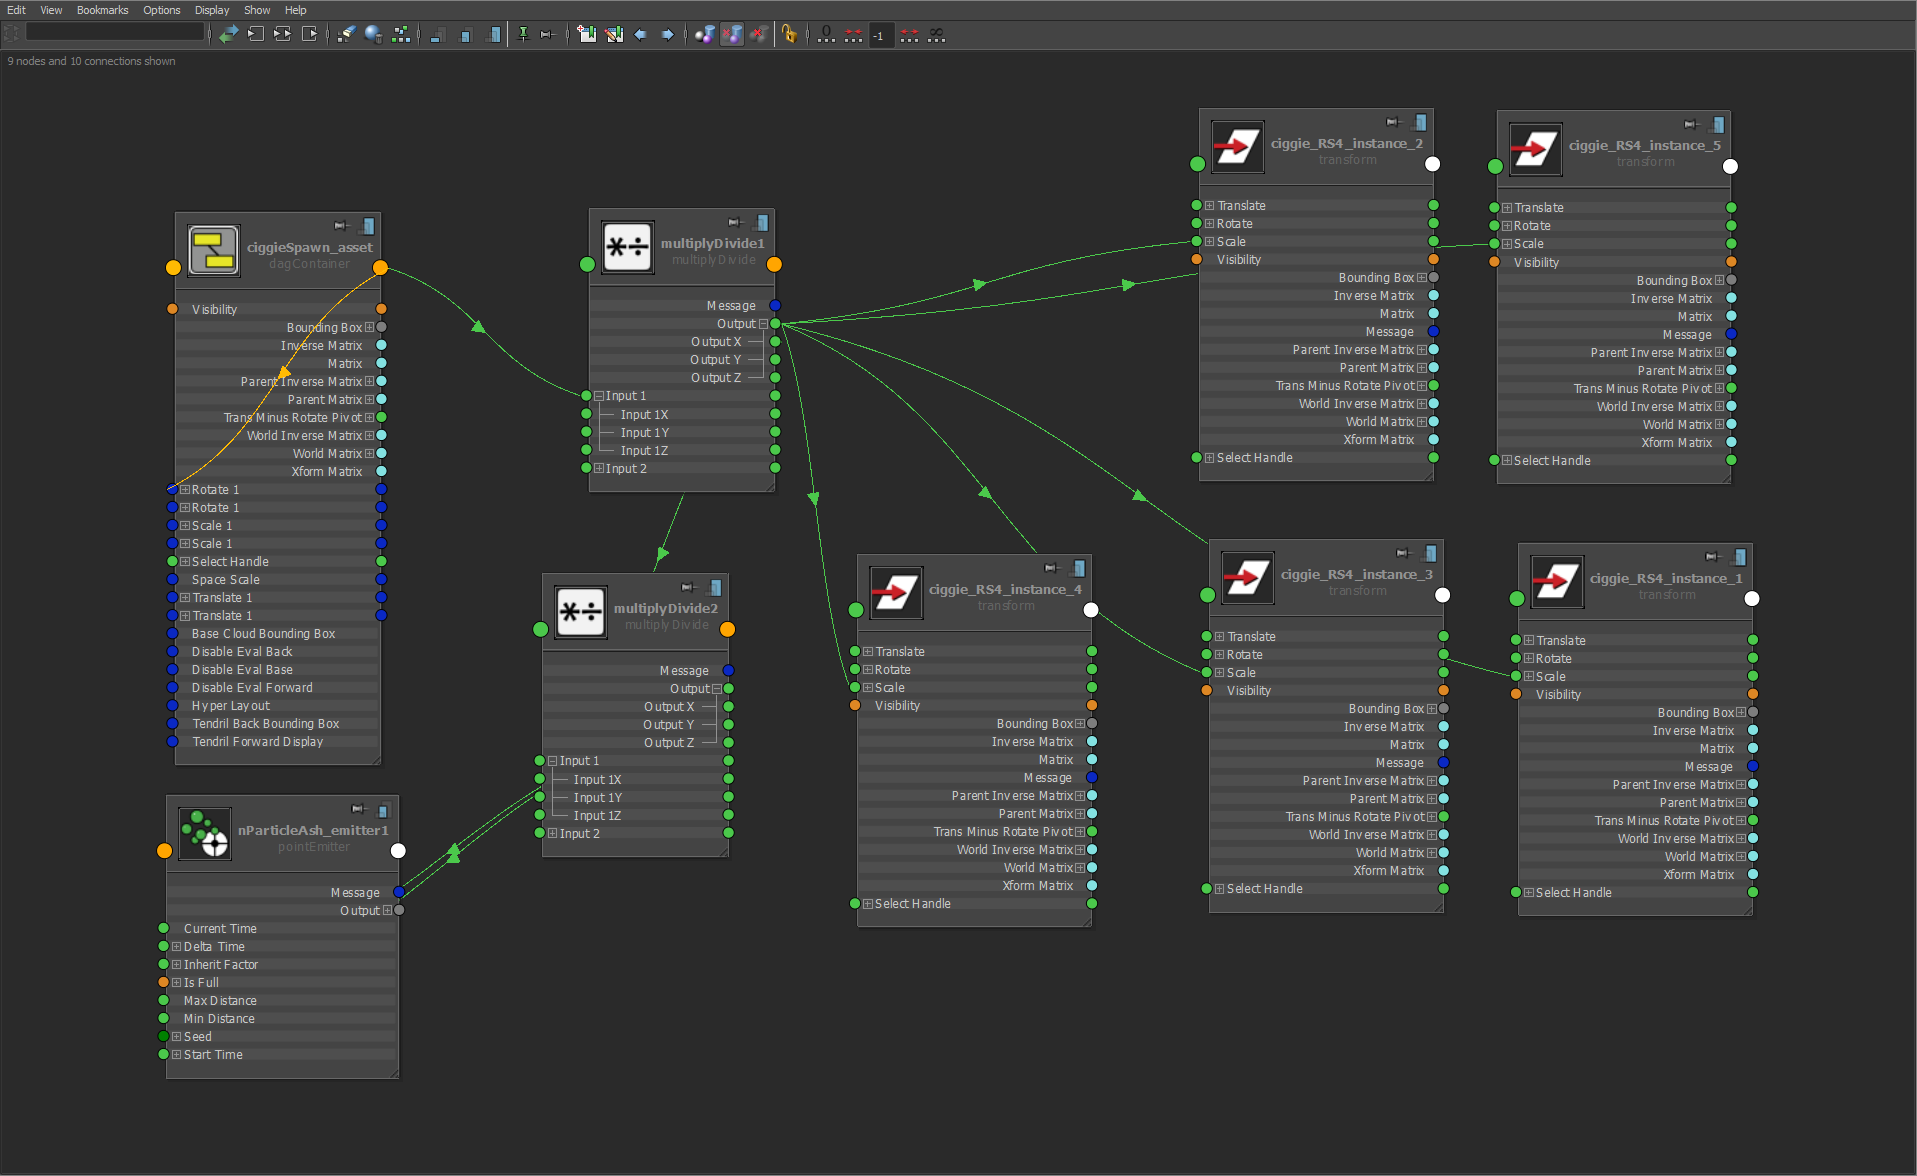
\includegraphics[width=\textwidth]{figures/node-based-editor}
    % forrás: https://3dpalmieri.wordpress.com/2012/09/13/dynamics-and-visual-effects-studio-2/
    \caption{Vizuális, csomópont alapú szerkesztő a Maya 3D modellezőben}
    \label{figure:node-based-editor}
\end{figure}

Sajnos a dolgozat kereteibe nem fért bele egy ilyen eszköz kifejlesztése, ezért egy egyszerűbb megoldást kellett választanom.
A jelenlegi interfész a feladatban található blokkokat egymás alatt jeleníti meg, az összeköttetések pedig név alapján válnak követhetővé.
A szerkesztő az elérhető opciók felsorolásával igyekszik segíteni a felhasználók munkáját.

A feladatok készítésének első lépése, hogy létrehozzuk és elnevezzük az új feladatot.
Ezután a \ref{figure:jporta-exercise}. ábrán látható nézet fogad minket, ahol kialakíthatjuk a feladat belső struktúráját.
Egy lenyitható részben találjuk a hozzáadható blokktípusok listáját.
A feladatban lévő blokkokat dobozok reprezentálják, amelyek bal oldalán sorakoznak bemeneteik, jobb oldalán kimeneteik, középen pedig az egyéb tulajdonságaik.
A blokkok összekötését a felhasználni kívánt kimenetek elnevezésével, majd a megfelelő bemeneteknél ezen nevek kiválasztásával tehetjük meg.

\begin{figure}[h]
    \centering
    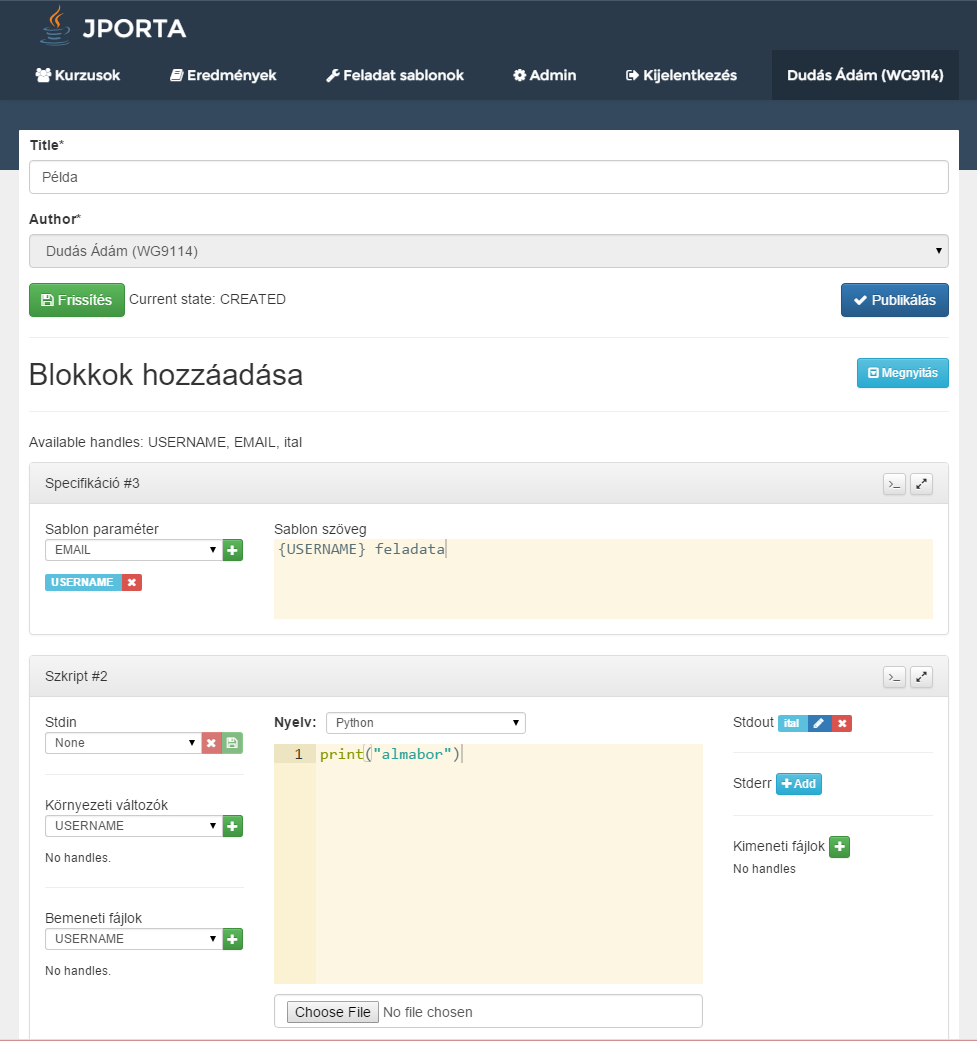
\includegraphics[width=\textwidth]{figures/jporta-exercise}
    \caption{Feladattervező nézet a Jportán}
    \label{figure:jporta-exercise}
\end{figure}

\section{Feladatok kiadása}
Miután a feladatok elkészültek, nincs más hátra, mint kiadni őket a hallgatóknak.
Ehhez két dologot kell megtennie az oktatónak: egyrészt véglegesíteni kell a feladatot, másrészt hozzá kell rendelni azt a hallgatók egy csoportjához.
Az előbbi a \ref{figure:jporta-exercise}. ábrán is látható \textbf{Publikálás} gombbal tehető meg a feladat szerkesztő nézetében.
Erre szintén két okból van szükség.
Egyrészt, ilyenkor végzi el a rendszer a feladat konzisztencia-ellenőrzését: minden kötelező mező kitöltésre került-e, nincs-e a függőségi gráfban kör, stb.
Másrészt, ekkor a feladat véglegesítésre kerül, ezután a lépés után nem lehet további változtatásokat végezni rajta egészen addig, míg visszavonásra nem kerül.
Ez azért nagyon fontos, mert a feladat bármilyen jellegű módosítása érvénytelenné tehetné a feladatra már beérkezett megoldásokat.

Publikálás után a feladat megjelenik a kiadható feladatok listájában, ahhonnan az oktató kiválaszthatja és hozzárendelheti egy kurzushoz vagy kurzuscsoporthoz.
Az összerendeléskor a feladat kiválasztásán túl egy nevet és egy határidőt is meg kell adni.
A feladat és a kiadás különválasztása azért fontos, mert így egy feladatot többször is fel lehet használni, akár különböző kurzusokban vagy szemeszterekben.

\section{Feladatbeadás}\label{section:submission}
A kiadott feladatok megjelennek a rendszerben a hallgatók számára, akik beadásokat készíthetnek ezekre.
Ha a feladat tartalmaz specifikációt, annak kiértékelése a feladatkiadás első megtekintésekor esedékes.
A hallgatók a feladatkiírás alapján elkészítik megoldásaikat, majd a felületen feltöltik a szükséges fájlokat.
Ekkor létrejön a \ref{figure:exercise-uml-cd}. ábrán látható \texttt{Submission} osztály egy egyede, amely összekapcsolja a hallgató által készített állományokat, a feladatkiadást és magát a hallgatót.
A beadás állapota kezdetben \textit{Kiértékelés alatt} (\texttt{under\_evaluation}) lesz.
Ha a feladat tartalmaz kézi beavatkozást igénylő blokkot, ennek ``végrehajtása'' idejére a feladat \textit{Kézi beavatkozásra vár} (\texttt{waiting\_for\_input}) állapotba kerül.
A beadás kiértékelése \textit{Sikeres} (\texttt{successful}) vagy \textit{Sikertelen} (\texttt{failed}) állapotban érhet véget.

A hallgatók a feladatkiadás határidejének lejárta előtt többször is próbálkozhatnak a beadással, akár egy sikeres beadás után is van lehetőségük további javításra.
Beadott megoldásaikat visszamenőleg megtekinthetik a feladatkiadás részletező oldalán.

\section{Megoldások ellenőrzése és értékelése}\label{section:submission-evaluation}
A feladatkiértékelő rendszer második fő feladata a hallgatók által beadott megoldások kiértékelése.
Ahogy az előző szakaszban láthattuk, amikor a hallgató a webportálon beadja a megoldását, létrejön egy \texttt{Submission} típusú objektum, amely ezt a beadást szimbolizálja.
Emellett, a beadás részeként feltöltött fájlokat a rendszer eltárolja, de már nem az eredeti, feltöltéskori nevükkelel, hanem annak az azonosítónak a nevével, amelyen az egyes fájlok hivatkozhatóak.
Ha például a feladatban szereplő \texttt{UserFile} blokk \textit{output} nevű kimenetét egy \textit{dokumentáció} elnevezésű azonosítóhoz kapcsoljuk, akkor a fájl neve a fájlrendszerben \textit{dokumentáció} lesz.
Ez azért előnyös, mert így a későbbi fájleléréseknek nem kell egy táblából kiolvasniuk, hogy milyen fájlnév alatt találják meg a keresett erőforrást.
Ugyanakkor bizonyos esetekben szükség lehet a fájl eredeti nevére, például a beadás megtekintésénél zavaró lehetne a hallgató számára, ha az ő általa \textit{első\_specifikációm.docx} néven feltöltött fájlt \textit{dokumentum} fájlnévvel találná meg.
Ilyen jellegű metaadatok tárolására a rendszer a \textit{kiterjesztett fájlattribútumok} (\textit{extended file attributes}) fájlrendszer funkciót használja.
Ez azért praktikus, mert a fájlhoz kötődik, azzal együtt mozog, törlődik, így a konzisztencia megörzésére nem kell további erőforrásokat fordítani.
Ezt a funkciót nagyon sok rendszer támogatja, hátránya viszont, hogy csak limitált mennyiségű adat (körülbelül pár 10 kilobájt) tárolására képes, ami azonban a mi esetünkben bőven elégséges. \cite{wiki:ExtendedFileAttributes}
% xattr: portal fs vs. backup fs támogatja-e

A beadások ezután bekerülnek a kiértékelő modul várakozási sorába aszinkron feldolgozásra, ezzel biztosítva a webportál minél kisebb késleltetését.
Ez a feldolgozási sor a jelenlegi rendszerben Celery segítségével kerül megvalósításra.

A Celery egy Pythonban íródott, nyílt forrású, aszinkron feladatvégrehajtásra specializálódott szoftver, mely elosztott üzenetküldési képességekkel is rendelkezik, ezáltal távoli eljáráshívás implementációjára is alkalmas.
A feladatok végrehajtását a Celery konkurrensen végzi, mégpedig úgy, hogy továbbítja azokat egy vagy több feldolgozófolyamatnak (\textit{worker process}), melyek akár különböző gépeken is elhelyezkedhetnek, teljesítve ezáltal a \ref{section:requirements}. szakaszban említett \ref{req:distributed}. követelményt.
A feldolgozók futhatnak egy, de akár többszálon is, illetve felhasználhatják az eventlet vagy gevent Python-alapú korutin függvénykönyvtárakat is.
A Celery az elosztott üzenetküldés funkciót többféle bróker felhasználásával is meg tudja valósítani, amelyek lehetnek AMQP (pl. RabbitMQ, ZeroMQ), kulcs--érték adatbázis (pl. Redis, MongoDB) vagy relációs adatbázis (SQLAlchemy, Django ORM) alapúak is.
A Jporta esetében a leginkább ajánlott RabbitMQ Advanced Message Queuing Protocol-t megvalósító bróker szoftvert válaszottam az üzenetek szétosztására a végpontok között. \cite{wiki:Celery} \cite{Celery}

A kiértékelő modul ezt a beadásokkal teli várakozási sort dolgozza fel, az egyes feladatok kiértékelését pedig a \ref{section:execution-procedure}. szakaszban leírt módon végzi.
Ilyenkor a folyamat a feladatban található \texttt{SubmissionResult} blokktól indul, ami a feladat eredményét reprezentálja, hiszen ez az, aminek az értékére szükségünk van.
A kiértékelés során minden érintett blokk \texttt{evaluate} metódusa meghívásra kerül, mégpedig egy \texttt{EvaluationContext} típusú paraméterrel.
Ez a ``kiértékelési környezet'' tartamazza a szükséges információkat a kiértékelés végrehajtásához.
A kontextuson keresztül érhetőek el a hallgató által feltöltött fájlok, a hallgató adatai, vagy más külső erőforrás.

Az \texttt{evaluate} metódus törzsében további aszinkron távoli eljáráshívások történhetnek, amelyek szintén Celery révén kerülnek elvégzése, ám ez már nem a feladatkiértékelő modul feladata, hanem a \textit{végrehajtó moduloké}.
A végrehajtó modulok implementálják az olyan fontos feladatokat, mint a forráskódok fordítása, futtatható állományok, szkriptek és tesztek futtatása.
A szükséges végrehajtó modulok a feladatokban felhasznált blokkok implementációjától függenek, magától a kiértékelő modultól, annak működésétől függetlenek, így részletes tárgyalásuk túlmutat a dolgozat keretein.

Az akár helyben, szinkron módon, akár a végrehajtó modulok által máshol, aszinkron módon elvégzett számítások eredményeit -- \textit{termékeit} -- a kiértékelő modul az \texttt{Artifact} osztály felhasználásával tárolja el.
Az \texttt{Artifact} osztály a blokkok kiértékelésének ``melléktermékeit'' szimbolizálja.
Az osztály példányosításához egy azonosítóra és egy kontextusra van szükség, amelyek tartalmazzás a szükséges információt az állományok eléréséhez.
Ahhoz, hogy ezeket a termékeket egyértelműen azonosítani tudja a rendszer, a következő információkra van szüksége:
\begin{itemize}
    \item a feladat egyedi azonosítója,
    \item a feladatkiadás egyedi azonosítója,
    \item az azonosító neve, amellyel a feladatban a termékre hivatkozunk,
    \item ha rendelkezésre áll, a beadás egyedi azonosítója,
    \item ha rendelkezésre áll, a kiértékelést indítványozó felhasználó egyedi azonosítója.
\end{itemize}
Az opcionálisan megjelölt adatok nem minden kiértékelésnél állnak rendelkezésre, például a feladatkiírás kiértékelésénél beadás még nem létezik, így ehhez nem köthető erőforrás.
Ezeken túl az azonosító -- az őt előállító kimenet beállítása révén -- meghatározza a termék tárolásának módját is.
Vannak olyan termékek, amelyek perzisztens tárolására nincs szükség, ezért elég, ha a memóriában helyezzük el őket, más termékeket viszont indokolt lehet fájlokban vagy adatbázisban tárolni.
Az előbbi kategóriába eső termékeket a Jporta egy Redis tárolóban helyezi el, utóbbiakat rendre a fájlrendszerben vagy a Django által felügyelt relációs adatbázisban.

A Redis egy C nyelven ír, nyílt forráskódú, memóriabeli kulcs--adatszerkezet tároló, amely használható adatbázisként, gyorsítótárként vagy -- az előzőekben már említett -- üzenet brókerként is.
\cite{Redis}
A Jporta implementációjánál kiváló gyorsítótár tulajdonsága, és átfogó utasításkészlete miatt választottam.

% Fejlesztés menete: git, Vim, CIRCLE devenv

\section{Összegzés}
Ebben a fejezetben prezentáltam a Jporta új feladatkiértékelő alrendszerének tervezési lépéseit.
Bemutattam, hogyan képes a rendszer feladatok leírására, illetve minként állíthatóak össze benne új feladatok.
Ezután röviden leírtam a feladatkiadás és -beadás működését, hogy végül eljuthassunk a beadások kiértékelésének problémájához.
Az általam vázolt megoldás ugyan megvalósítja az elvárt funkcionalitást, de a dolgozat írásának idején még közel sem tekinthető késznek.

A funkció csak kezdetlegesen került beágyazásra a Jporta felületébe, továbbá véleményem szerint a \ref{section:exercise-creation}. szakaszban vázolt vizuális szerkesztőeszköz sokat javítana a feladatkészítés folyamatának ergonómiáján.
Hiányos még a rendelkezésre álló blokkok listája is, amelyek sokszor félkész megoldásként szolgálhatnának a feladatok összeállításánál.
Elkészült azonban a blokkok egy minimális csoportja, amelyeket a következő szakasz részletez.

\subsection{Elkészült blokkok}
Ebben a szakaszban sorraveszem és röviden bemutatom a dolgozat befejezéséig elkészült blokktípusokat.

\subsubsection{AuthorFile}
\textbf{Leírás:} a feladat szerzője által feltöltött fájlt tartalmazó blokk \\
\textbf{Tulajdonságok:} -- \\
\textbf{Bemenetek:} -- \\
\textbf{Kimenetek:}
\begin{itemize}
    \item output: a szerző által feltöltött fájl tartalma
\end{itemize}
        
\subsubsection{Checker}
\textbf{Leírás:} a megoldáson futtatott tesztek eredményét egyszerű sablon-behelyettesítéssel vizsgáló blokk \\
\textbf{Tulajdonságok:}
\begin{itemize}
    \item expected: az elvárt eredmény sablonja, melybe a \texttt{params} bemenet értékeit behelyettesítve kapjuk meg az elvárt eredményt
\end{itemize}
\textbf{Bemenetek:}
\begin{itemize}
    \item actual: a teszt lefutása során kapott eredmény
    \item params: az elvárt eredmény sablonjába behelyettesítendő értékek
\end{itemize}
\textbf{Kimenetek:}
\begin{itemize}
    \item result: az ellenőrzés eredménye
\end{itemize}

\subsubsection{DefaultValue}
\textbf{Leírás:} a végrehajtási kontextusban alapból elérhető értékeket szolgáltató blokk \\
\textbf{Tulajdonságok:} -- \\
\textbf{Bemenetek:} -- \\
\textbf{Kimenetek:}
\begin{itemize}
    \item email: az éppen kiértékelt megoldás szerzőjének e-mail címe
    \item username: az éppen kiértékelt megoldás szerzőjének felhasználóneve
\end{itemize}

\subsubsection{GccCompiler}
\textbf{Leírás:} egy forrásfájl fordítást végző blokk, ami a GCC fordítót használja \\
\textbf{Tulajdonságok:}
\begin{itemize}
    \item extra\_arguments: tetszőleges egyéb parancssori argumentumokat tartalmazó sztring a fordító számára
\end{itemize}
\textbf{Bemenetek:}
\begin{itemize}
    \item files\_in: egyéb bemeneti fájlok, melyeket a fordítási folyamat felhasználhat
    \item libraries: függvénykönytárak
    \item sources: fordítandó forrásfájlok
    \item stdin: szabványos bemenet
\end{itemize}
\textbf{Kimenetek:}
\begin{itemize}
    \item files\_out: egyéb kimeneti fájlok, melyek a fordítás során keletkeztek vagy módosultak
    \item runnable: a fordítás során keletkezett futtatható állomány
    \item stderr: szabványos hibakimenet
    \item stdout: szabványos kimenet
\end{itemize}

\subsubsection{LecturerApproval}
\textbf{Leírás:} valamilyen eredmény oktató által történő kézi értékelését jelző blokk \\
\textbf{Tulajdonságok:} -- \\
\textbf{Bemenetek:}
\begin{itemize}
    \item dependencies: azok az értékek, amelyekre a kézi értékeléshez szükség van
\end{itemize}
\textbf{Kimenetek:}
\begin{itemize}
    \item result: a kézi értékelés eredménye
\end{itemize}

\subsubsection{Runner}
\textbf{Leírás:} futtatható állomány futtatását végző blokk \\
\textbf{Tulajdonságok:} -- \\
\textbf{Bemenetek:}
\begin{itemize}
    \item environment: környezeti változók a futtatás során
    \item files\_in: bemeneti fájlok, melyeket a futtatott állomány felhasználhat
    \item runnable: a futtatandó állomány
    \item stdin: szabványos bemenet
\end{itemize}
\textbf{Kimenetek:}
\begin{itemize}
    \item files\_out: kimeneti fájlok, melyek a futás során keletkeztek vagy módosultak
    \item stderr: szabványos hibakimenet
    \item stdout: szabványos kimenet
\end{itemize}

\subsubsection{Script}
\textbf{Leírás:} a feladat létrehozásakor megadott szkriptet futtató blokk \\
\textbf{Tulajdonságok:}
\begin{itemize}
    \item language: a programnyelv, amelyen a szkript íródott
\end{itemize}
\textbf{Bemenetek:}
\begin{itemize}
    \item environment: környezeti változók a futtatás során
    \item files\_in: bemeneti fájlok, melyeket a futtatott szkript felhasználhat
    \item stdin: szabványos bemenet
\end{itemize}
\textbf{Kimenetek:}
\begin{itemize}
    \item files\_out: kimeneti fájlok, melyek a futás során keletkeztek vagy módosultak
    \item stderr: szabványos hibakimenet
    \item stdout: szabványos kimenet
\end{itemize}

\subsubsection{Specification}
\textbf{Leírás:} feladat specifikációját megadó blokk \\
\textbf{Tulajdonságok:}
\begin{itemize}
    \item template\_text: a specifikáció szövegének sablonja
\end{itemize}
\textbf{Bemenetek:}
\begin{itemize}
    \item template\_params: a specifikáció szövegének sablonjába behelyettesítendő értékek
\end{itemize}
\textbf{Kimenetek:} --

\subsubsection{SubmissionResult}
\textbf{Leírás:} a feladatra adott megoldás eredményét megadó blokk \\
\textbf{Tulajdonságok:} -- \\
\textbf{Bemenetek:}
\begin{itemize}
    \item source: a megoldás eredménye
\end{itemize}
\textbf{Kimenetek:} --

\subsubsection{UserFile}
\textbf{Leírás:} a hallgató által a megoldásához feltöltött fájlt tartalmazó blokk \\
\textbf{Tulajdonságok:}
\begin{itemize}
    \item allowed\_extensions: a feltöltött fájl engedélyezett kiterjesztései
    \item size\_limit: a feltölthető fájl maximális mérete
\end{itemize}
\textbf{Bemenetek:} -- \\
\textbf{Kimenetek:}
\begin{itemize}
    \item output: a hallgató által feltöltött fájl tartalma
\end{itemize}

%----------------------------------------------------------------------------
\chapter{Javaslat további funkciókra}\label{chapter:features}
%----------------------------------------------------------------------------
Diplomaterv feladatkiírásom része, hogy tegyek javaslatot olyan új modulokra vagy módosításokra, melyekkel a Jporta funkcionalitása bővíthető lenne.
A portál fejlesztése közben sok hasznos ötlet látott napvilágot.
Ebben a fejezetben az általam leghasznosabbnak ítélt két funkció indokoltságát foglalom össze, illetve vázolom egy lehetséges megvalósításukhoz szükséges tervezési és implementációs lépéseket.

\section{Csapatrendszer}
Az első javaslatom egy csapatmunka támogatását lehetővé tevő funkció Jportába történő integrálása lenne.
A csapatrendszer feladata, hogy lehetővé tegye hallgatói csapatok kialakítását mind hallgatók, mind oktatók által, illetve a Jporta meglévő adminisztrációs funkcióit (értékelés, jelenlét, stb.) kiterjessze egyéni hallgatókról csapatokra.

A Jporta fejlesztésének megkezdésekor felmerült IIT-n használt egyéb, hasonló célú, oktatási rendszerek konszolidációja az új portálba, amivel a sok különböző alkalmazás működtetésére, karbantartására szánt idő és erőforrások csökkenthetőek lennének.
Az egyik ilyen rendszer a Hercules, melynek többek között a Szoftver projekt laboratórium -- régi nevén Szoftver labor 4. -- tárgy oktatásában van szerepe.
A tárgy keretében a hallgatók csapatban végzik el egy kisebb komplexitású szoftver tervezését, fejlesztését és dokumentálását.
A Hercules egyik legfontosabb funkciója is ehhez kapcsolódik, mégpedig hogy a félév elején biztosítja a hallgatók számára az említett csapatok kialakítását.
A jelenlegi rendszerben a hallgatóknak egy hét áll rendelkezésére a félév elején, hogy önállóan kialakítsák az 5-6 főből álló csapatokat, melyeket a Hercules felületén regisztrál a csapat vezetője.
A csapat regisztrációjakor meg kell adnia a csapat egyedi nevét, a csapattagok pedig a Neptun kódjukkal kerülnek azonosításra.
A határidő letelte után csapat nélkül maradt hallgatókat a tárgy felelőse osztja be csapatokba saját belátása szerint. 

\subsection{Tervezés}
A tervezés első lépése a Hercules fent leírt funkciójának megismerése és az új rendszerhez való illesztési lehetőségeinek vizsgálata.
Ezután következhet csak egy új, csapatokat modellező osztály és a hozzá kapcsolódó üzleti logika megvalósítását segítő segédosztályok definiálása, továbbá a már meglévő kódrészek hozzáigazítása az új fejlesztéshez.

A csapatrendszer egyik alapvető funkciója a csapatok kialakítása.
A Hercules által implementált metódus kissé körülményes, kevés rugalmasságot biztosít a felhasználók számára.
Ezért az új rendszerben ennek a funkciónak némi átalakítással, modernizálással kell megvalósulni, igazodva a Jporta adottságaihoz, és kihasználva azokat.

A csapatalakítás menete az új rendszerben lehetne a következő:
\begin{enumerate}
    \item A hallgató belép a portálra és kiválasztja a tárgyat, amelyhez csapatot kíván alakítani.
    \item Kiválasztja az \textit{Új csapat alakítása} funkciót és megadja a csapat nevét.
    \item A létrejött csapatba meginvitálja hallgatótársait, amiről azok értesítést kapnak a Jporta beépített üzenetküldő rendszerén keresztül.
    \item A csapat meghívott tagjai eldöntik, hogy elfogadják-e a meghívást.
\end{enumerate}
Ebben az elgondolásban a csapatot létrehozó hallgató tölti be a csapatkapitány szerepét, ezért neki -- a csapatalakítás időszakában -- lehetősége van a csapatból csapattagok eltávolítására, illetve új csapattagok meghívására.
A csapatkapitány mindenképp részét képezi a csapatnak.
Minden hallgató tárgyanként legfeljebb egy csapatnak lehet tagja.
Azok a hallgatók, akik már tagjai egy csapatnak, de nem kapitányai csapatuknak, megszüntethetik tagságukat, és ezután van lehetőségük új csapatba invitációt elfogadni, vagy saját csapatot létrehozni.

A tárgy adatlapján az oktató megadhatja, hogy a tárgyban csapatmunka támogatására van-e szükség, és ha igen, akkor milyen alsó és felső korlát van a csapatok méretére, illetve mely időtartományban van lehetősége a hallgatóknak csapatot alakítani.
A tárgy oktatóinak bármikor lehetősége van új csapat létrehozására, illetve a meglévő csapatok törlésére, módosítására, de fontos, hogy ezzel a jogosultságukkal csak indokolt esetben éljenek.
Különös figyelmet kell fordítani a hallgatók csapatok közti mozgatására, mivel ez egy igen gyakori művelet, ami kitüntetett támogatás nélkül nehézkes és időigényes feladattá tud válni.

A csapatrendszer bevezetése miatt a portál megjelenésének és kezelésének is változnia kell.
Az oktatók egy tárgy adatlapján eddig az egyes hallgatókat értékelhették, adminisztrálhatták az órákon való részvételüket, adhattak ki nekik feladatot.
Az új rendszerben viszont, a csapatmunkát igénylő tárgyaknál ezeknek a funkcióknak csapatokon kell elvégezhetőeknek lenniük.

\subsection{Megvalósítás}
A csapatrendszer implementálásának alapja a csapatot megtestesítő Django modell létrehozása.
Ez az osztály írja le, milyen attribútumok tárolódnak az egyes csapatokról az adatbázisban, illetve hogy a Jporta rendszerének többi entitásával milyen kapcsolatban áll (lásd \ref{figure:teams-after}. ábra).
Ugyanez az osztály implementálja a csapatokhoz szorosan kapcsolódó üzleti logikát is.
Ahogy az a \ref{figure:teams-before}. és \ref{figure:teams-after}. ábra összehasonlításából jól látszik, a változtatások után a felhasználót reprezentáló \texttt{SwdUser} osztályt sok esetben a \texttt{Team} osztály váltja fel, ugyanakkor a tervezésnél már említettem, hogy a csapatok használata tárgyanként eltérő lehet, egy kapcsolótól függ csupán, melyet a tárgy oktatója választ meg.
Ezt a kettősséget úgy oldanám fel, hogy a háttérben mindkét esetben csapatokkal dolgozik a modell, ám ha az adott tárgy nem igényel csapatmunka-támogatást, akkor a rendszer minden felhasználó számára automatikusan létrehozza a felhasználó egyszemélyes csapatát.
A felhasználók számára ez egy teljesen transzparens folyamat, a megjelenítés a tárgyhoz beállítása alapján dönti el, hogy csapatok vagy egyéni felhasználók megjelenítésére van-e szükség egy adott esetben.

\begin{figure}[h]
    \centering
    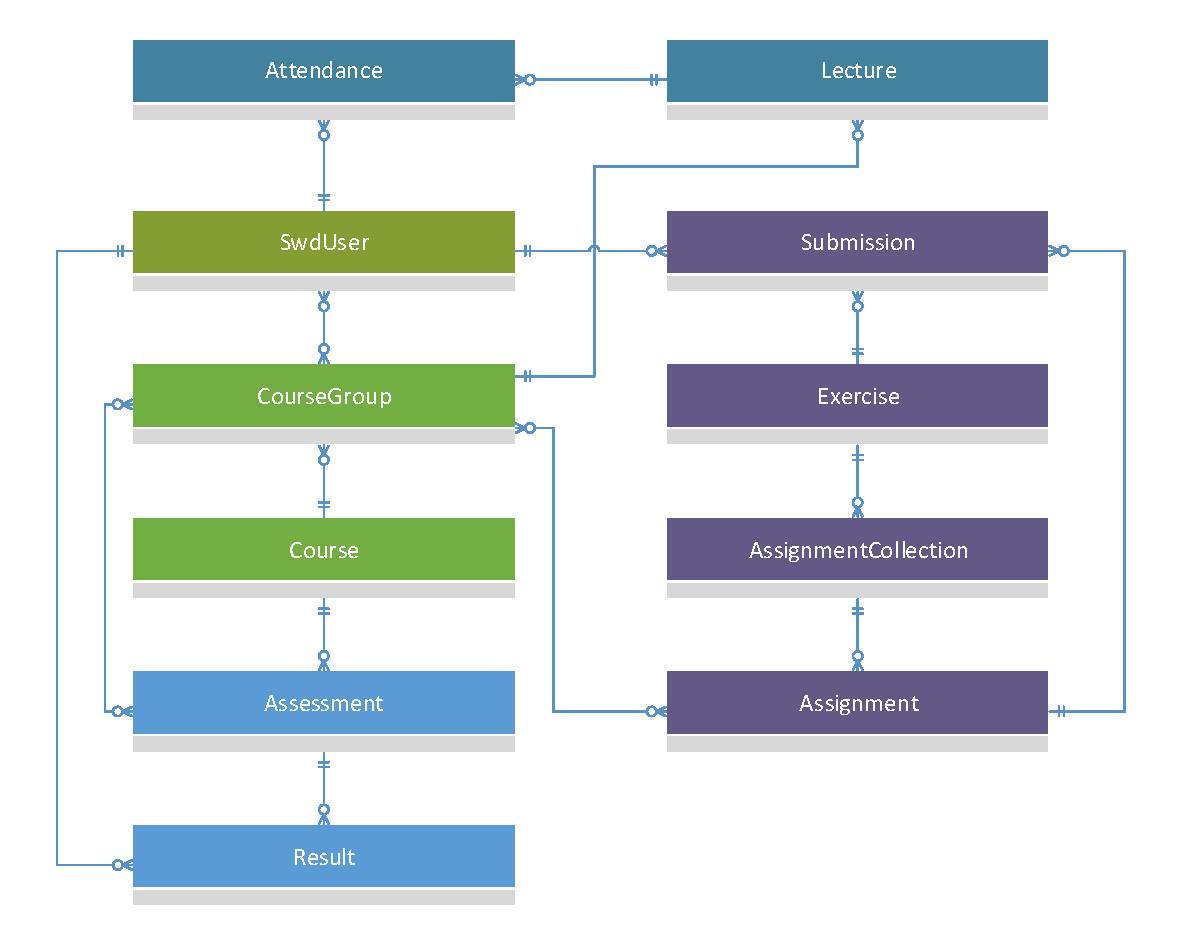
\includegraphics[width=\textwidth]{figures/teams-before}
    \caption{Jporta modellje csapatok nélkül}
    \label{figure:teams-before}
\end{figure}

\begin{figure}[h]
    \centering
    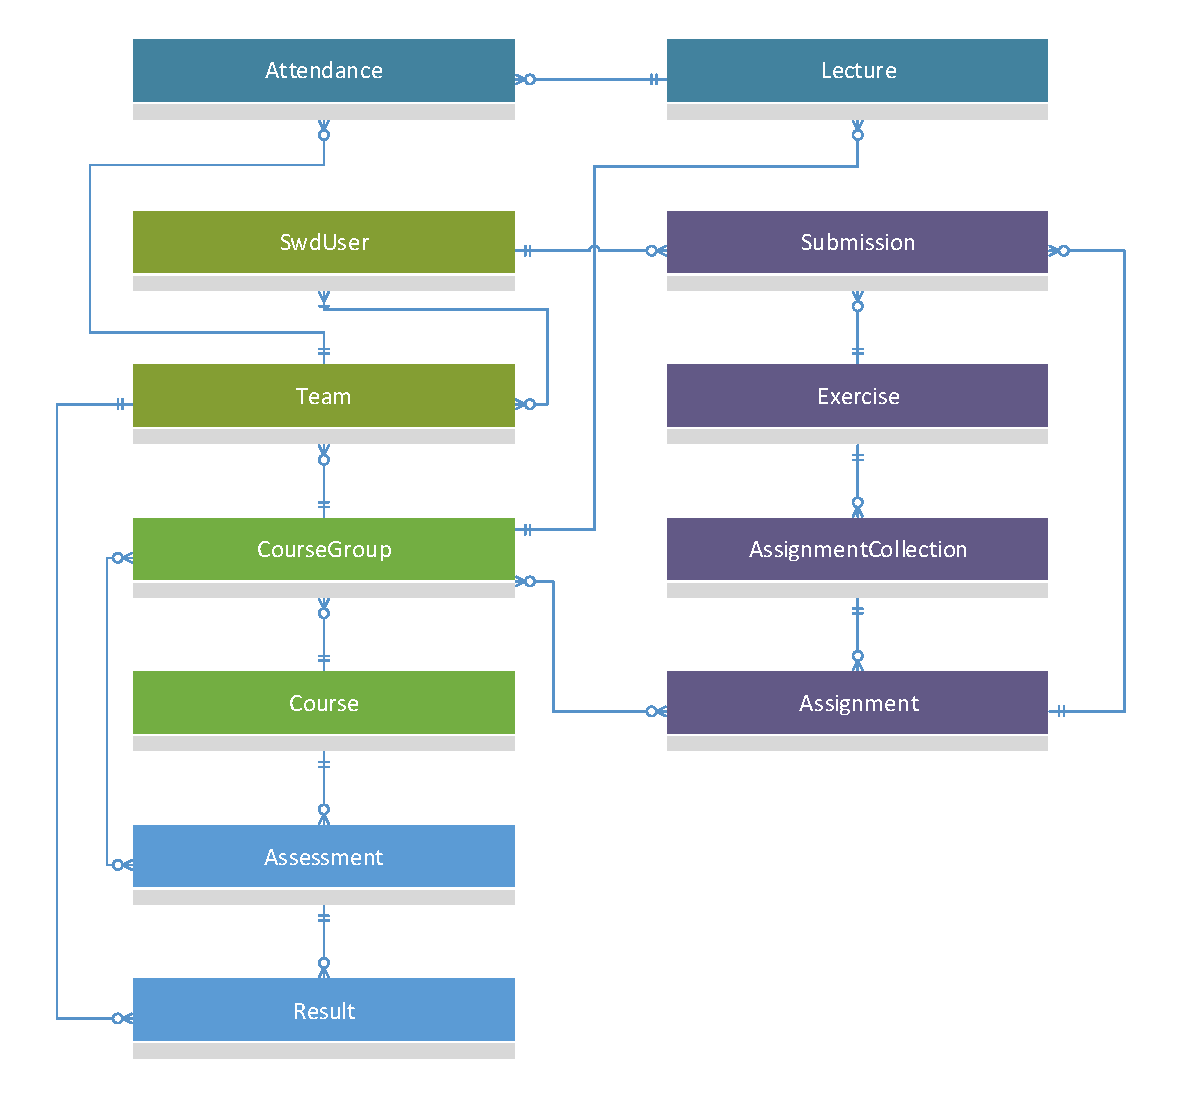
\includegraphics[width=\textwidth]{figures/teams-after}
    \caption{Jporta modellje csapatokkal}
    \label{figure:teams-after}
\end{figure}

További változás, hogy az eddig a kurzuscsoportok tagjainak nyilvántartására használt, Djangoba beépítetten érkező \texttt{Group} osztályt a fejlesztés során ki kell váltani egy több-több kapcsolatot nyilvántartó ``kapcsolótáblával'', mivel az egyes kurzuscsoportok (\texttt{CourseGroup}) most már nem felhasználóhoz (\texttt{SwdUser}), hanem csapatokhoz (\texttt{Team}) kapcsolódnak, ezeknek a tárolását viszont a \texttt{Group} osztály nem támogatja.

\section{Integráció verziókövető rendszerrel}
A második javaslatom egy olyan funkció beépítésére vonatkozik, amely lehetővé tenné, hogy a hallgatók egy verziókezelő szoftver segítségével tudják beadni megoldásaikat.
Ezzel a hallgatók a verziókövető rendszerek használatát a szoftverfejlesztéssel egybekötve sajátíthatnák el, ami egyrészt jó habitus, másrészt követi a valódi fejlesztés menetét.

A verziókezelő rendszerek alapvető megértése és használatuk elsajátítása szinte minden szoftverfejlesztő számára nélkülözhetetlen.
A általunk létrehozott állományok különböző állapotainak tárolása több előnnyel is jár.
Például könnyedén megtudhatjuk, mi változott a legutóbbi állapot óta, vagy akár két régebbi állapot között.
Ezt a tudást felhasználhatjuk akár egyfajta munkanaplóként is, vagy bármikor könnyedén visszaállíthatunk felülírt vagy törölt részeket.

\subsection{Tervezés}
Az első lépés egy megfelelő verziókövető rendszer kiválasztása, majd eztután következhet az integráció részleteinek tervezése.

A változáskövető rendszerek manapság két nagy csoportra oszthatók: \textit{központi} (\textit{centralized}, pl. CVS, SVN, TFS) és \textit{elosztott} (\textit{distributed}, pl. Bazaar, Git, Mercurial).
Kezdetben a fejlesztők központi verziókezelő rendszereket készítettek és használtak, mivel így volt a legegyszerűbb a tartalmak megosztása, ezáltal a közös munka.
Az utóbbi 10 év során azonban az elosztott rendszerek fokozatosan, de egyértelműen átvették a vezetést, köszönhetően a könnyen hozzáférhető interneteléréseknek, és a nyílt forráskódú szoftvereknél gyakori közösségi fejlesztés elterjedésének, melynek magasfokú párhuzamosság-igényével a központi rendszerek nem tudnak megbirkózni.
A központi verziókövetők legnagyobb hátránya az elosztottakkal szemben, hogy utóbbiak képesek szimulálni az előbbiek egy szerver--több kliens konfigurációját, de emellett sokkal nagyobb rugalmasságot és több funkciót biztosítanak.
Ezen okok miatt én egy elosztott verziókezelő rendszert, a Gitet választanám.

A Gitet 2005-ben Linus Torvalds készítette a Linux kernel fejlesztéséhez, de azóta napjaink egyik legelterjedtebb megoldásává vált.
A Git alapvető használata a parancssorból sem túlzottan bonyolult -- köszönhetően egyszerű felépítésének --, de létezik sok grafikus alkalmazás is\footnote{Egy átfogó listáért lásd: \url{https://git.wiki.kernel.org/index.php/Interfaces,\_frontends,\_and\_tools\#Graphical\_Interfaces}}, melyekkel kezdők és profik egyaránt könnyedén elboldogulnak, sőt, minden elterjedtebb integrált fejlesztőkörnyezet tartalmaz Gitet támogató beépülő modulokat.
A Git emellett gyors, biztonságos, és a legtöbb operációs rendszeren támogatott.

Ahogy más elosztott verziókezelő rendszerekben, a Gitben is különválik a \textit{commitolás} -- a fájlok pillanatnyi állapotának rögzítése --, és a \textit{pusholás} -- a létrejött commitok publikálása, megosztása -- művelete.
A fejlesztő egy feladat megoldása közben tetszőleges számú commitot készíthet, ám ezekről mások csak akkor értesülnek, amikor a fejlesztő egy távoli tárolóval szinkronizál, megosztja a változásait: pushol.

A portálnak tehát biztosítania kell egy verziókezelt tárolót a hallgató számára, amelybe feltöltheti megoldásait a változáskövető rendszer segítségével.
Amikor a hallgató ebbe a tárolóba feltölti legújabb megoldását, a Jportában keletkeznie kell egy beadásnak a fájlok legfrissebb állapotát felhasználva.

Mivel a Jportát több hallgató is használja, továbbá egy hallgató több feladatra is küld be megoldásokat, felmerülhet a kérdés, hogy hány tárolóra van ekkor szükség összesen?
A Git képes egy tárolón belül több különböző fejlesztési ág -- \textit{branch} -- párhuzamos menedzselésére is.
Ezt felhasználva akár egyetlen tároló is elegendő lenne, ha minden felhasználó--feladatkiadás páros számára külön ágat hozunk létre.
Ennek a rendszernek a használata azonban körülményes és ellenkezik a megszokott használati mintákkal is.
Az egy tárolós megoldás és a másik véglet -- vagyis hogy minden felhasználó minden feladatához külön tárolót biztosítunk -- között több változat is elképzelhető, ám véleményem szerint ez utóbbi a legelőnyösebb választás, mégpedig azért, mert így a hallgatók egy majdnem teljes értékű verziótároló szolgáltatást vehetnek igénybe a portálon.

Néhány megkötést azonban mégis tenni kell a tároló használatával kapcsolatban.
Az egyik megkötés, hogy a beadórendszer csak egy kitüntetett -- pl. \textit{master} -- ág módosításait figyeli, így a hallgató a valódi fejlesztéseknél is alkalmazott sémát követhet a verziókövető használatakor.
A másik megkötés, hogy ezen az ágon nem engedélyezett az úgynevezett \textit{forced push} művelet, vagyis az ág történelmének felülírása, mivel ez inkonzisztens állapotba hozhatná a portált -- pl. eltűnhet olyan állapot, amiből beadás készült.

A Git több protokollt is támogat a tárolók közötti kommunikációra.
Ezek közül nekünk olyanra van szükségünk, amely támogatja a felhasználók azonosítását, mert csak így érhetjük el, hogy kizárólag a Jporta felhasználói érhessék el a tárolókat, illetve minden felhasználó csak a saját tárolóihoz férjen hozzá.
A két szóbajövő protokoll a HTTPS és az SSH.
Mindkét protokoll biztonságos és ajánlott, különösebb hátránnyal egyik sem rendelkezik.
A legnagyobb eltérés a kettő között az azonosítás módjában rejlik.
Míg a HTTPS protokoll használatakor a HTTP-nél megszokott azonosítási módszerek legtöbbje alkalmazható (pl. felhasználónév--jelszó páros), addig SSH fölött kizárólag SSH kulcspárral azonosíthatja magát a felhasználó.
\cite{ProGit}

A Git működéséről és használatáról bővebb információkat \cite{ProGit} ad. 

\subsection{Megvalósítás}
Az integráció megvalósításához egy kapcsolat létrehozására van szükség a verziókövető és a Jporta között.
A verziókövetőnek tudnia kell jelezni a portálnak, amikor új beadás történt, a portálnak pedig hozzá kell tudnia férni a verziókezelő által tárolt adatokhoz.

A kapcsolat első irányát, vagyis az új verziók érkezésének jelzését, a Git \textit{hook} funkciójával lehetne megvalósítani.
A hookok olyan programok, amelyeket a Git valamilyen esemény hatására automatikusan lefuttat.
Az egyik ilyen hook a \textit{post-update hook}, amelyet a \textit{git-reveive-pack} hív meg a -- küldő szempontjából -- távoli tárolón, miután a frissítés befejeződött.
Ezt a működést a helyi gépen kiadott \texttt{git push} parancs idézi elő, vagyis pontosan akkor történik, mikor a felhasználó szinkronizálni szeretné változásait a Jportával.
\cite{GitHooks}
A Jporta esetében a hook által végrehajtott program lehetne egy egyszerű -- például Python nyelvű -- szkript, ami a webportálon beadott megoldások regisztrációjával analóg műveletet hajt végre.
A programot a Git tároló gyökerében található \texttt{hooks} könyvtárban kell elhelyezni \texttt{post-update} névvel.  % `git rev-parse --git-dir`/hooks/post-update vagy `git config core.hooksPath`/post-update, ha felül van írva
Ezenkívül az állománynak futtathatónak kell lennie a Git műveleteket végző felhasználó által.

Ahhoz, hogy a portál ezután hozzá tudjon férni a verziókövetőben tárolt adatokhoz, a pygit2 függvénykönyvtár használatát javasolnám.
Ez a függvénykönyvtár a libgit2 megosztott könyvtárhoz biztosít hozzáférést Python nyelvből, így a fontosabb Git műveletek elvégezhetőek segítségével. \cite{pygit2}

A hallgatók és a Jportán lévő verziókezelt tárolók összekapcsolását az előző szakaszban ismertetett protokollokon keresztül valósítanám meg.
Mielőtt viszont a hallgató publikálhatná megoldásait a portálra, szükség van a verziókezelt tárolók létrehozására az adott felhasználó--feladatkiadás páros számára.
A tárolók automatikus létrehozása feleslegesen terhelheti a portál erőforrásait, hiszen nem biztos, hogy minden hallgató minden feladatához használni fogja ezt a lehetőséget, ezért jobb megoldás lehet, ha a hallgatóknak a webportálon maguknak kell indítványozniuk a tároló létrehozását minden feladatkiadás esetén.
Ez a felfogás összhangban van a legtöbb verziókövető, illetve más verziótároló szolgáltatást nyújtó portálok -- pl. BitBucket, GitHub -- működésével is.
%----------------------------------------------------------------------------
\chapter*{Összefoglalás}\addcontentsline{toc}{chapter}{Összefoglalás}
%----------------------------------------------------------------------------

A megtervezett műszaki alkotás értékelése, kritikai elemzése, továbbfejlesztési lehetőségek

\section*{További fejlesztések}\addcontentsline{toc}{section}{További fejlesztések}
%----------------------------------------------------------------------------
\chapter*{Köszönetnyilvánítás}\addcontentsline{toc}{chapter}{Köszönetnyilvánítás}
%----------------------------------------------------------------------------

Szeretnék köszönetet mondani konzulensemnek, Dr.~Szeberényi Imrének, aki tanulmányaimban és munkám során is támogatott engem -- és rajtam kívül még egy másik tucat hallgatót -- áldozatos munkájával.  

Külön köszönet jár kollégámnak, Kálmán Viktornak, akivel vállvetve dolgoztunk a Jporta rendszer tervezésén és megvalósításán, és aki nélkül a Jporta kezelői felületének ergonómiája egy kaktuszéval vetekedne.

Köszönet illeti Őry Mátét és Guba Sándort, akiknek a Jporta alapjainak lerakásában volt fontos szerepe, valamint a BME IK többi munkatársát, akik kellemesebbé tették a munkával eltöltött időt.

Végül, de nem utolsó sorban, szeretném megköszönni édesapámnak, Dr.~Dudás Lászlónak és páromnak, Szabó Katalinnak, hogy a munka és jelen dolgozat megírása alatt végig segítettek és támogattak. 
\listoffigures\addcontentsline{toc}{chapter}{Ábrák jegyzéke}
\listoftables\addcontentsline{toc}{chapter}{Táblázatok jegyzéke}
%\printglossary[title=Rövidítések jegyzéke]

\bibliography{bibliography}\addcontentsline{toc}{chapter}{Irodalomjegyzék}
\bibliographystyle{huplain}

\label{page:last}
\end{document}
